% ====================================================================================
\chapter{有限元方法：能量极小化}
% ====================================================================================

\section*{引言：从飞机到桥梁}

1943年，第二次世界大战正酣。英国工程师们面临一个紧迫的问题：如何计算新型飞机机翼的应力分布？机翼形状复杂，传统的解析方法根本无法应对。

\storynote{Richard Courant}{1888--1972，德裔美国数学家，有限元方法的先驱。纳粹上台后逃离德国，在纽约大学创建了著名的库朗数学研究所(Courant Institute)。他与希尔伯特合著的《数学物理方法》至今仍是经典教材。}

数学家 Richard Courant 提出了一个革命性的想法：与其求解整个连续体的方程，不如把机翼\textbf{切成很多小三角形}，在每个三角形内假设应力是简单的（比如线性的），然后把这些小块``拼起来''。

这个想法就是\textbf{有限元方法}（Finite Element Method，FEM）的雏形。不过“有限元”这个名字要到 1960 年才由 Ray Clough 在论文里首次使用；在那之前的 1956 年，Turner、Clough、Martin 和 Topp 已经为波音的机翼分析发展出了刚度法——“刚度”这个词，我们很快就会在刚度矩阵里再遇到。

\begin{figure}[htbp]
\centering
\begin{tikzpicture}[scale=0.9]
    % 定义机翼形状的上下边界函数
    % 上边界: y_top(x) 从(0,0)到(6,0.15)，中间凸起
    % 下边界: y_bot(x) 从(0,0)到(6,0.15)，中间凹陷

    % 填充三角形网格 - 手动绘制以确保填满
    \begin{scope}
        \clip (0,0) .. controls (1.5,0.7) and (4,0.55) .. (6,0.15) --
              (6,0.15) .. controls (4,-0.15) and (1.5,-0.25) .. (0,0);

        % 绘制三角形网格
        \foreach \i in {0,1,...,11} {
            \foreach \j in {0,1,...,3} {
                \pgfmathsetmacro{\x}{\i*0.5}
                \pgfmathsetmacro{\y}{\j*0.25 - 0.25}
                % 上三角形
                \draw[gray!60, thin] (\x,\y) -- (\x+0.5,\y) -- (\x+0.25,\y+0.25) -- cycle;
                % 下三角形
                \draw[gray!60, thin] (\x+0.25,\y+0.25) -- (\x+0.5,\y) -- (\x+0.5,\y+0.25) -- cycle;
            }
        }
    \end{scope}

    % 机翼轮廓（加粗）
    \draw[very thick, blue!70!black] (0,0) .. controls (1.5,0.7) and (4,0.55) .. (6,0.15);
    \draw[very thick, blue!70!black] (0,0) .. controls (1.5,-0.25) and (4,-0.15) .. (6,0.15);

    % 标注
    \node at (3,-1) {机翼被切成很多小三角形单元};

    % 放大一个单元
    \begin{scope}[shift={(8,0)}]
        \draw[thick, fill=blue!15] (0,0) -- (1.5,0) -- (0.75,1) -- cycle;
        \fill[red] (0,0) circle (2.5pt);
        \fill[red] (1.5,0) circle (2.5pt);
        \fill[red] (0.75,1) circle (2.5pt);
        \node at (0.75,-0.5) {一个三角形单元};
        \node[right, font=\small] at (1.6,0) {节点};
        \draw[<-, thick] (1.55,0.05) -- (1.9,0.3);
    \end{scope}
\end{tikzpicture}
\caption{有限元方法的基本思想：把复杂形状切成简单的小块}
\end{figure}

\subsection*{有限元的现代应用}

1967 年，Zienkiewicz 出版了第一本有限元专著。今天，有限元方法已是工程计算的绝对基石：建筑工程用它计算桥梁、高楼的应力分布以确保结构安全，汽车工业用它模拟碰撞测试、优化车身设计，航空航天用它分析飞机机翼与火箭发动机的热应力，电子产品用它模拟芯片散热与电磁场分布，医学用它分析人工关节的力学性能、模拟心脏血流。
\clarify{为什么这一章放在“物理智能”部分，而不是紧跟第5章的力学？因为它真正的下游是第14章的 PINN 和第15章的神经算子：要把物理定律嵌进神经网络，先得知道物理是怎么被算出来的——弱形式、刚度矩阵、条件数，都会在那两章原样出现。它只依赖第3章的变分法和第5章的最小作用量，可以随时回来读。}

\begin{example}[你身边的有限元]
你的手机外壳在设计前，工程师用有限元模拟过跌落时的应力；港珠澳大桥在建造前，工程师用有限元分析过风载和车载下的变形；波音787的机翼用复合材料，设计全靠有限元优化。
\end{example}

\vspace{0.5cm}
\noindent\textit{为什么一台连微分方程都不会解的计算机，能算出机翼上每一点的应力？为什么把区域切成三角形之后，问题反而变简单了？为什么工程师说“固定端的支反力”，数学家却说“边界条件的乘子”？}

\begin{quote}
\textbf{本章目标}：让你看清一个事实——工程师用来算桥梁、飞机的有限元软件，骨子里做的就是第1章那件事：写下一个能量（目标函数），把边界条件当约束，求导等于零。唯一的新东西是“把无限维的函数切成有限个帐篷”。读完本章，你应该能徒手算出一个刚度矩阵，并且说得清 $\lambda$ 为什么是边界上的热流或支反力。
\end{quote}

\subsection*{本章的核心观点}

令人惊讶的是，这个强大的工程工具的数学本质就是我们已经学过的\textbf{变分法的离散化}：

\begin{tcolorbox}[colback=yellow!10, colframe=orange!80, title=核心观点]
\textbf{有限元不是什么新东西——它就是第1章的拉格朗日乘子法，只不过变量从几个数变成了成千上万个节点值。}目标函数是总势能 $J(U) = \frac{1}{2}U^\top KU - F^\top U$，约束是“边界上的值被钉死”，求导等于零就得到 $KU = F$。这里 $K$ 是刚度矩阵，描述系统的“硬度”；$U$ 是我们要求的未知量——节点处的位移、温度或电势；$F$ 是载荷向量，代表外部作用力、热源或电荷。

\begin{center}
\renewcommand{\arraystretch}{1.3}
\small
\begin{tabular}{lll}
\toprule
 & \textbf{第1章} & \textbf{本章（有限元）} \\
\midrule
变量 & $x \in \R^n$ & 节点值 $U \in \R^n$（离散化的 $u(x)$） \\
目标 & $f(x)$ & 总势能 $J(U) = \frac{1}{2}U^\top KU - F^\top U$ \\
约束 & $g(x) = 0$ & Dirichlet 边界条件 $BU = g$ \\
乘子 & $\lambda$（影子价格） & $\lambda$ = 边界热流 / 支反力 \\
一阶条件 & $\nabla f + \lambda \nabla g = 0$ & $KU + B^\top \lambda = F$，$BU = g$ \\
\bottomrule
\end{tabular}
\end{center}
\end{tcolorbox}
\review{第3章}{还记得变分法吗？我们把连续曲线离散成$y_0, y_1, \ldots, y_N$，把积分变成求和，把泛函极值问题变成有限维优化问题。有限元方法用的是完全相同的套路！}

\begin{tcolorbox}[colback=green!5, colframe=green!60!black, title=学完这章，你将能够...]
\begin{itemize}
    \item 把Poisson方程转化为能量最小化问题（变分形式）
    \item 手算一维有限元问题的刚度矩阵和载荷向量
    \item 用Python/MATLAB组装刚度矩阵并求解$KU=F$
    \item 理解工程软件（ANSYS、COMSOL）背后的数学原理
    \item 估算网格密度与计算精度的关系
\end{itemize}
\end{tcolorbox}

% ------------------------------------------------------------------------------------
\section{从物理问题到数学方程}

\subsection{一个简单的例子：一维热传导}

想象一根长度为 1 米的金属棒，两端固定在 0°C 的冰水中，中间有一个均匀的热源（比如电流通过产生的焦耳热）。问：稳态时棒上的温度分布是什么？

\begin{figure}[htbp]
\centering
\begin{tikzpicture}[scale=1.0]
    % 金属棒
    \fill[gray!30] (0,-0.3) rectangle (6,0.3);
    \draw[thick] (0,-0.3) rectangle (6,0.3);
    
    % 边界条件
    \fill[blue!30] (-0.5,-0.5) rectangle (0,0.5);
    \fill[blue!30] (6,-0.5) rectangle (6.5,0.5);
    \node at (-0.25,0.8) {\small 0°C};
    \node at (6.25,0.8) {\small 0°C};
    
    % 热源
    \foreach \x in {1,2,3,4,5} {
        \draw[red, thick, ->] (\x,-0.8) -- (\x,-0.4);
    }
    \node[red] at (3,-1.2) {均匀热源 $f$};
    
    % 温度分布（虚线）
    \draw[blue, thick, dashed] plot[smooth] coordinates {(0,0.3) (1,0.8) (2,1.1) (3,1.2) (4,1.1) (5,0.8) (6,0.3)};
    \node[blue] at (3,1.5) {温度分布 $u(x)$};
    
    % 坐标
    \node at (0,-0.6) {\small $x=0$};
    \node at (6,-0.6) {\small $x=1$};
\end{tikzpicture}
\caption{一维热传导问题}
\end{figure}

\subsection{Poisson方程从哪里来？}

在有限元和PINN中，你会反复遇到\textbf{Poisson方程}（泊松方程）。让我们从物理第一性原理推导它。
\preview{第14章的 PINN 也要解同一个 Poisson 方程，只是把这里的“形函数”换成神经网络。学完本章再看第14章，你会发现两者只差一个“基函数怎么选”。}

\begin{keyidea}[Poisson方程的推导——大白话版]
\textbf{核心物理}：守恒律 + 本构关系 = 偏微分方程

\textbf{步骤1：守恒律}

考虑热传导。取一小段$[x, x+\Delta x]$，稳态下热量``流进 + 生成 = 流出''：
\[
q(x) + f(x)\Delta x = q(x + \Delta x)
\]
其中$q(x)$是热流密度（单位时间流过$x$处的热量，向右为正），$f(x)$是热源强度。

整理得：$\frac{q(x+\Delta x) - q(x)}{\Delta x} = f(x)$

当$\Delta x \to 0$：
\[
\frac{dq}{dx} = f(x) \quad \text{（守恒律：热流的增量来自热源）}
\]

\textbf{步骤2：本构关系（傅里叶定律）}

热量从高温流向低温，流速与温度梯度成正比：
\[
q = -k\frac{du}{dx} \quad \text{（傅里叶定律）}
\]
这里$k$是热导率（设$k=1$简化），负号表示热量流向温度降低的方向。

\textbf{步骤3：合并}

把傅里叶定律代入守恒律：
\[
\frac{d}{dx}\left(-\frac{du}{dx}\right) = f(x) \quad \Rightarrow \quad \boxed{-\frac{d^2u}{dx^2} = f(x)}
\]

这就是一维Poisson方程！高维情况只需把$\frac{d^2}{dx^2}$换成Laplacian算子$\nabla^2$：
\[
-\nabla^2 u = f \quad \text{（Poisson方程）}
\]
\end{keyidea}

\subsection{现实问题与PDE的对应关系}

Poisson方程（及其变种）描述了惊人多的物理现象：

\begin{center}
\renewcommand{\arraystretch}{1.4}
\begin{tabular}{l|l|l|l}
\toprule
\textbf{物理问题} & \textbf{方程} & \textbf{$u$代表} & \textbf{$f$代表} \\
\midrule
稳态热传导 & $-\nabla^2 u = f$ & 温度 & 热源强度 \\
静电场 & $-\nabla^2 \phi = \rho/\varepsilon_0$ & 电势 & 电荷密度 \\
万有引力 & $\nabla^2 \phi = 4\pi G\rho$ & 引力势 & 质量密度 \\
弹性膜变形 & $-\nabla^2 u = f$ & 挠度 & 压力 \\
地下水渗流 & $-\nabla \cdot (K\nabla h) = Q$ & 水头 & 源/汇 \\
\midrule
\multicolumn{4}{c}{\textit{时间相关的方程}} \\
\midrule
热扩散 & $\frac{\partial u}{\partial t} = \alpha \nabla^2 u$ & 温度 & — \\
波动 & $\frac{\partial^2 u}{\partial t^2} = c^2 \nabla^2 u$ & 位移 & — \\
Schrödinger & $i\hbar\frac{\partial \psi}{\partial t} = -\frac{\hbar^2}{2m}\nabla^2\psi + V\psi$ & 波函数 & 势能 \\
Navier-Stokes & $\rho(\frac{\partial \vec{v}}{\partial t} + \vec{v}\cdot\nabla\vec{v}) = -\nabla p + \mu\nabla^2\vec{v}$ & 速度场 & 压力 \\
\bottomrule
\end{tabular}
\end{center}

\begin{insightbox}
\textbf{为什么这么多问题都对应类似的方程？}因为它们都遵循相同的模式：一条\textbf{守恒律}（能量、质量或电荷守恒），加上一条\textbf{本构关系}（流量与梯度成正比，即 Fourier、Ohm 或 Darcy 定律）。这就是为什么学会用有限元解一个问题（如热传导），就等于学会了解\textbf{所有}类似问题！
\end{insightbox}

\subsection{物理定律：热传导方程}

根据上面的推导，稳态温度分布 $u(x)$ 满足：

\begin{equation}
-\frac{d^2 u}{dx^2} = f(x), \quad x \in (0, 1)
\end{equation}

加上边界条件：
\begin{equation}
u(0) = 0, \quad u(1) = 0
\end{equation}

这里 $u(x)$ 是位置 $x$ 处的温度，是我们要求的未知函数；$f(x)$ 是已知的热源强度；$-\frac{d^2u}{dx^2}$ 则是热量的“净流出率”。

\paragraph{物理直觉}

方程 $-u'' = f$ 说的是：在稳态下，热源产生的热量等于热传导带走的热量。如果 $u'' < 0$，温度曲线开口向下、像山峰，热量就从这点向两边流出；如果 $u'' > 0$，温度曲线开口向上、像山谷，热量就从两边流入这点。稳态要求流入等于流出加上热源产生的量，这正是方程两边所表达的平衡。

\subsection{这个方程能解析求解吗？}

对于简单情况（如 $f = $ 常数），可以直接积分两次：

\begin{example}[$f = 1$ 的解析解]
\begin{align}
-u'' &= 1 \\
\Rightarrow \quad u' &= -x + C_1 \\
\Rightarrow \quad u &= -\frac{x^2}{2} + C_1 x + C_2
\end{align}

代入边界条件 $u(0) = 0$ 得 $C_2 = 0$；$u(1) = 0$ 得 $C_1 = \frac{1}{2}$。

所以解析解是：
\[
u(x) = \frac{x(1-x)}{2}
\]
这是一条开口向下的抛物线，最高点在 $x = 0.5$ 处，$u_{\max} = 0.125$。
\end{example}

\textbf{但是}，在实际工程问题中，区域形状可能很复杂（如飞机机翼），材料可能不均匀（$f$ 是复杂函数），边界条件也可能很复杂。这时解析解不存在，必须用数值方法——这就是有限元！

% ------------------------------------------------------------------------------------
\section{变分原理：换一个角度看问题}

\subsection{从微分方程到能量最小化}

上一节的结尾留下了一个困难：微分方程要求在每一点都成立，形状一复杂就无从下手。既然逐点求解走不通，能不能换一种提法，把“每点都满足方程”改写成“某个整体的量取最小”？第3章和第5章告诉我们，很多微分方程可以从变分原理推导出来。热传导方程也不例外！

\begin{keytheorem}[title=能量原理]
定义\textbf{能量泛函}：
\begin{equation}
J[u] = \frac{1}{2}\int_0^1 (u')^2 \, dx - \int_0^1 f \cdot u \, dx
\end{equation}

则：
\begin{equation}
u^* = \arg\min_u J[u] \quad \Longleftrightarrow \quad -u^{*\prime\prime} = f
\end{equation}

即：\textbf{求解微分方程} $\Leftrightarrow$ \textbf{找使能量最小的函数}
\end{keytheorem}

\paragraph{能量泛函的物理意义}

第一项 $\frac{1}{2}\int (u')^2 dx$ 是\textbf{内能}，与温度梯度的平方成正比；第二项 $\int fu \, dx$ 是\textbf{外部热源的“功”}；两者相减，$J$ 就是内能减去外功，即总势能。系统自然趋向于总势能最小的状态——这就是能量最小化原理！
\think{能量泛函里为什么是 $-\int fu\,dx$ 而不是 $+\int fu\,dx$？提示：把 $f$ 想成重力、$u$ 想成位移，外力做功会降低系统的势能。}

\subsection{验证：从变分到微分方程}

让我们用第3章的 Euler-Lagrange 方程验证这个等价性。

泛函：$J[u] = \int_0^1 F(x, u, u') \, dx$，其中 $F = \frac{1}{2}(u')^2 - fu$

计算偏导数：
\[
\frac{\partial F}{\partial u} = -f, \quad \frac{\partial F}{\partial u'} = u'
\]

E-L 方程：
\[
\frac{\partial F}{\partial u} - \frac{d}{dx}\frac{\partial F}{\partial u'} = 0 \quad \Rightarrow \quad -f - u'' = 0 \quad \Rightarrow \quad -u'' = f
\]

确实得到了热传导方程！

\begin{insightbox}
\textbf{两种视角的等价性}：

\begin{center}
\begin{tabular}{c|c}
\textbf{微分方程视角} & \textbf{变分视角} \\
\hline
找满足 $-u'' = f$ 的函数 & 找使 $J[u]$ 最小的函数 \\
\hline
局部条件（每点都要满足） & 整体条件（能量最小） \\
\hline
需要解微分方程 & 需要做优化 \\
\end{tabular}
\end{center}

有限元方法从变分视角出发——因为优化问题更容易离散化！
\end{insightbox}

% ------------------------------------------------------------------------------------
\section{弱形式：降低光滑性要求}

\subsection{强形式的困难}

微分方程 $-u'' = f$ 叫做\textbf{强形式}，因为它要求 $u$ 在每个点都精确满足，而且 $u$ 必须有二阶导数。

但在实际问题中，解可能不够光滑：材料交界处（如铜棒接钢棒）温度梯度可能不连续，集中热源处温度分布可能有“尖角”。这些地方二阶导数并不存在，强形式无从谈起，于是我们需要一种对光滑性要求更低的写法。

\subsection{弱形式：用积分代替微分}

\textbf{弱形式}用一个巧妙的技巧绕过了光滑性问题：

\begin{enumerate}
    \item 把方程两边乘以一个\textbf{测试函数} $v(x)$
    \item 对整个区间积分
    \item 用分部积分把导数“转移”到测试函数上
\end{enumerate}

\paragraph{推导过程}

从强形式出发：
\[
-u'' = f
\]

乘以测试函数 $v$，积分：
\[
-\int_0^1 u'' \cdot v \, dx = \int_0^1 f \cdot v \, dx
\]

对左边用分部积分：
\[
-\int_0^1 u'' v \, dx = -[u' v]_0^1 + \int_0^1 u' v' \, dx
\]

如果测试函数 $v$ 在边界上为零（$v(0) = v(1) = 0$），边界项消失：

\begin{keyformula}[title=弱形式]
找 $u$ 使得对所有满足 $v(0) = v(1) = 0$ 的测试函数 $v$：
\begin{equation}
\boxed{\int_0^1 u' \cdot v' \, dx = \int_0^1 f \cdot v \, dx}
\end{equation}
\end{keyformula}

\clarify{“弱”不是“不严格”。弱形式的解若恰好足够光滑，它一定也满足强形式；反过来，材料交界处梯度不连续的解只满足弱形式。弱形式是“更宽容”，不是“更马虎”。}

\paragraph{弱形式的优点}

弱形式带来三样好处。首先它\textbf{降低了光滑性要求}：只需要 $u$ 有一阶导数，不需要二阶导数，前面说的材料交界处于是不再是障碍。其次它\textbf{自然地处理边界条件}：某些边界条件会在分部积分的边界项里自动满足。最后它\textbf{便于离散化}：下一节将看到，从弱形式可以直接导出有限元方程。

\begin{physicalmeaning}
弱形式的物理意义是\textbf{能量平衡}：

左边 $\int u' v' dx$ 可以理解为“虚位移 $v$ 产生的内部虚功”

右边 $\int fv dx$ 是“外力对虚位移做的虚功”

弱形式说：对任意虚位移，内部虚功 = 外部虚功（虚功原理）
\end{physicalmeaning}

% ------------------------------------------------------------------------------------
\section{有限元离散化}

\subsection{核心思想：用有限维逼近无限维}

弱形式是一个关于函数 $u(x)$ 的方程——$u$ 有无限多个自由度（每个点的值都是未知的）。

有限元的核心思想是：用有限个\textbf{基函数}的线性组合来逼近真实解：
\begin{equation}
u_h(x) \approx U_1 \phi_1(x) + U_2 \phi_2(x) + \cdots + U_n \phi_n(x) = \sum_{j=1}^n U_j \phi_j(x)
\end{equation}

其中 $\phi_j(x)$ 是预先选定的\textbf{形函数}，是已知的；$U_j$ 是待求的\textbf{系数}，是未知的；$n$ 是自由度数，而且是有限的。这样，无限维问题变成了求 $n$ 个未知数 $(U_1, U_2, \ldots, U_n)$ 的问题！

\subsection{形函数：有限元的“积木块”}

最常用的形函数是\textbf{分片线性函数}，也叫\textbf{帐篷函数}或\textbf{帽子函数}：

\begin{figure}[htbp]
\centering
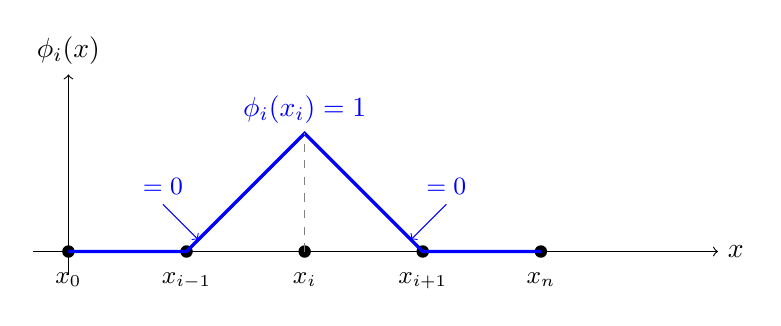
\begin{tikzpicture}[scale=1.5]
    % 坐标轴
    \draw[->] (-0.3,0) -- (5.5,0) node[right] {$x$};
    \draw[->] (0,-0.2) -- (0,1.5) node[above] {$\phi_i(x)$};
    
    % 网格节点
    \foreach \x/\lab in {0/$x_0$, 1/$x_{i-1}$, 2/$x_i$, 3/$x_{i+1}$, 4/$x_n$} {
        \fill (\x,0) circle (1.5pt);
        \node[below] at (\x,-0.1) {\small \lab};
    }
    
    % 形函数 φ_i
    \draw[very thick, blue] (0,0) -- (1,0) -- (2,1) -- (3,0) -- (4,0);
    
    % 标注
    \node[blue, above] at (2,1) {$\phi_i(x_i) = 1$};
    \draw[blue, <-] (1.1,0.1) -- (0.8,0.4) node[above] {\small $= 0$};
    \draw[blue, <-] (2.9,0.1) -- (3.2,0.4) node[above] {\small $= 0$};
    
    % 帐篷形状说明
    \draw[dashed, gray] (2,0) -- (2,1);
\end{tikzpicture}
\caption{帐篷函数 $\phi_i(x)$：在节点 $x_i$ 处等于 1，在相邻节点处等于 0，中间线性过渡}
\end{figure}

\paragraph{形函数的关键性质}

\begin{equation}
\phi_i(x_j) = \delta_{ij} = \begin{cases} 1, & i = j \\ 0, & i \neq j \end{cases}
\end{equation}

这个性质保证了：\textbf{系数 $U_i$ 恰好等于节点 $x_i$ 处的近似解值}！

验证：
\[
u_h(x_i) = \sum_j U_j \phi_j(x_i) = \sum_j U_j \delta_{ji} = U_i
\]

\subsection{从弱形式到线性方程组}

现在把近似解 $u_h = \sum_j U_j \phi_j$ 代入弱形式。

测试函数也用形函数：取 $v = \phi_i$（$i = 1, 2, \ldots, n$）

\paragraph{代入弱形式}

\[
\int_0^1 u_h' \cdot \phi_i' \, dx = \int_0^1 f \cdot \phi_i \, dx
\]

左边：
\[
\int_0^1 \left(\sum_j U_j \phi_j'\right) \phi_i' \, dx = \sum_j U_j \underbrace{\int_0^1 \phi_j' \phi_i' \, dx}_{K_{ij}}
\]

右边：
\[
\underbrace{\int_0^1 f \phi_i \, dx}_{F_i}
\]

于是得到：

\begin{keyformula}[title=有限元线性方程组]
\begin{equation}
\boxed{KU = F}
\end{equation}

其中 $K_{ij} = \int_0^1 \phi_i'(x) \phi_j'(x) \, dx$ 是\textbf{刚度矩阵}的元素，$F_i = \int_0^1 f(x) \phi_i(x) \, dx$ 是\textbf{载荷向量}的元素，$U = (U_1, U_2, \ldots, U_n)^\top$ 是待求的\textbf{节点值向量}。
\end{keyformula}

这就是有限元的核心方程！一个无限维的变分问题，变成了一个 $n \times n$ 的线性方程组。
\preview{本章“与优化的联系”一节会证明：$KU = F$ 正是 $J(U) = \frac{1}{2}U^\top KU - F^\top U$ 的一阶条件 $\nabla_U J = 0$——还是第1章“求导等于零”的老套路。}

% ------------------------------------------------------------------------------------
\section{刚度矩阵的计算}

\subsection{为什么叫“刚度矩阵”？}

“刚度”这个名字来自弹性力学。在弹簧系统中，$F = kx$，$k$ 是刚度——力与位移的比值。

在有限元中，$KU = F$ 说的是：\textbf{节点力 = 刚度矩阵 $\times$ 节点位移}。

$K_{ij}$ 的物理意义：给节点 $j$ 一个单位位移，节点 $i$ 受到多大的力？

\subsection{刚度矩阵的结构}

让我们计算刚度矩阵的元素 $K_{ij} = \int_0^1 \phi_i' \phi_j' dx$。

\paragraph{关键观察}

帐篷函数 $\phi_i$ 只在 $[x_{i-1}, x_{i+1}]$ 区间内非零（\textbf{局部支撑}）。因此，如果 $|i - j| > 1$，即节点不相邻，$\phi_i$ 和 $\phi_j$ 的支撑不重叠，积分自然为零，$K_{ij} = 0$；只有 $|i - j| \leq 1$，即相邻或相同节点时，$K_{ij} \neq 0$。这导致刚度矩阵是\textbf{稀疏的三对角矩阵}！

\begin{figure}[htbp]
\centering
\begin{tikzpicture}[scale=0.6]
    % 画一个 5x5 的矩阵
    \draw[gray] (0,0) grid (5,5);
    
    % 填充非零元素
    % 主对角线
    \foreach \i in {0,...,4} {
        \fill[blue!60] (\i,4-\i) rectangle ++(1,1);
    }
    % 上下对角线
    \foreach \i in {0,...,3} {
        \fill[blue!30] (\i+1,4-\i) rectangle ++(1,1);
        \fill[blue!30] (\i,3-\i) rectangle ++(1,1);
    }
    
    % 标注
    \node at (2.5,-1) {三对角矩阵};
    \node[right] at (5.5,4.5) {\small $K_{11}$};
    \node[right] at (5.5,3.5) {\small $K_{22}$};
    \draw[->] (5.3,2.5) -- (4.2,2.5);
    \node[right] at (5.5,2.5) {\small 对角线};
\end{tikzpicture}
\caption{一维有限元的刚度矩阵是三对角的：只有相邻节点之间有耦合}
\end{figure}

\subsection{具体计算刚度矩阵元素}

设网格是均匀的，步长为 $h = \frac{1}{N}$，节点为 $x_k = kh$（$k = 0, 1, \ldots, N$）。

\paragraph{情况1：对角线元素 $K_{ii}$（$i$ 和自己的耦合）}

$\phi_i$ 在 $[x_{i-1}, x_i]$ 上斜率为 $+\frac{1}{h}$，在 $[x_i, x_{i+1}]$ 上斜率为 $-\frac{1}{h}$。

\begin{figure}[htbp]
\centering
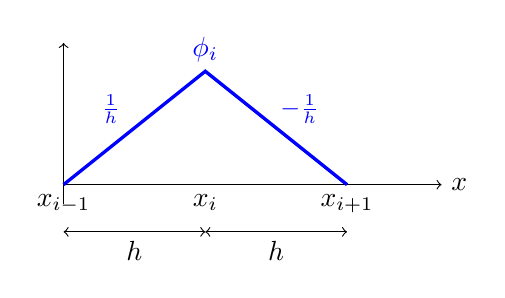
\begin{tikzpicture}[scale=1.2]
    \draw[->] (0,0) -- (4,0) node[right] {$x$};
    \draw[->] (0,-0.2) -- (0,1.5);
    
    % 形函数
    \draw[very thick, blue] (0,0) -- (1.5,1.2) -- (3,0);
    \node[blue, above] at (1.5,1.2) {$\phi_i$};
    
    % 斜率标注
    \node[blue] at (0.5,0.8) {\small $\frac{1}{h}$};
    \node[blue] at (2.5,0.8) {\small $-\frac{1}{h}$};
    
    % 节点
    \node[below] at (0,0) {$x_{i-1}$};
    \node[below] at (1.5,0) {$x_i$};
    \node[below] at (3,0) {$x_{i+1}$};
    
    % 区间标注
    \draw[<->] (0,-0.5) -- (1.5,-0.5) node[midway, below] {$h$};
    \draw[<->] (1.5,-0.5) -- (3,-0.5) node[midway, below] {$h$};
\end{tikzpicture}
\end{figure}

\begin{align}
K_{ii} &= \int_{x_{i-1}}^{x_{i+1}} (\phi_i')^2 \, dx \\
&= \int_{x_{i-1}}^{x_i} \left(\frac{1}{h}\right)^2 dx + \int_{x_i}^{x_{i+1}} \left(-\frac{1}{h}\right)^2 dx \\
&= \frac{1}{h^2} \cdot h + \frac{1}{h^2} \cdot h = \frac{2}{h}
\end{align}

\paragraph{情况2：相邻元素 $K_{i,i+1}$（相邻节点的耦合）}

$\phi_i$ 和 $\phi_{i+1}$ 只在 $[x_i, x_{i+1}]$ 上同时非零。

\begin{figure}[htbp]
\centering
\begin{tikzpicture}[scale=1.8]
    % 坐标轴
    \draw[->] (-0.3,0) -- (4.5,0) node[right] {$x$};
    \draw[->] (0,-0.2) -- (0,1.5) node[above] {};
    
    % 网格节点
    \foreach \x/\lab in {0/$x_{i-1}$, 1.5/$x_i$, 3/$x_{i+1}$, 4.5/$x_{i+2}$} {
        \fill (\x,0) circle (1.5pt);
    }
    \node[below] at (0,-0.1) {\small $x_{i-1}$};
    \node[below] at (1.5,-0.1) {\small $x_i$};
    \node[below] at (3,-0.1) {\small $x_{i+1}$};
    \node[below] at (4.2,-0.1) {\small $x_{i+2}$};
    
    % 形函数 φ_i (蓝色)
    \draw[very thick, blue] (0,0) -- (1.5,1.2) -- (3,0);
    \node[blue, above left] at (1.5,1.2) {$\phi_i$};
    
    % 形函数 φ_{i+1} (红色)
    \draw[very thick, red] (1.5,0) -- (3,1.2) -- (4.2,0);
    \node[red, above right] at (3,1.2) {$\phi_{i+1}$};
    
    % 重叠区域高亮
    \fill[purple, opacity=0.15] (1.5,0) -- (3,0) -- (3,1.2) -- (1.5,1.2) -- cycle;
    \fill[purple, opacity=0.15] (1.5,0) -- (1.5,1.2) -- (3,0) -- cycle;
    
    % 实际重叠的三角形区域（两个函数都非零的地方）
    \fill[green, opacity=0.2] (1.5,0) -- (2.25,0.6) -- (3,0) -- cycle;
    
    % 斜率标注
    \draw[blue, thick, ->] (2,0.4) -- (2.4,0.08);
    \node[blue] at (2.5,0.5) {\small $\phi_i' = -\dfrac{1}{h}$};
    
    \draw[red, thick, ->] (2.2,0.25) -- (2.6,0.57);
    \node[red] at (1.8,0.9) {\small $\phi_{i+1}' = +\dfrac{1}{h}$};
    
    % 区间标注
    \draw[<->, thick, purple] (1.5,-0.4) -- (3,-0.4);
    \node[purple, below] at (2.25,-0.4) {\small 重叠区间 $[x_i, x_{i+1}]$};
    
    % h 标注
    \draw[<->] (1.5,-0.7) -- (3,-0.7);
    \node at (2.25,-0.9) {\small $h$};
\end{tikzpicture}
\caption{相邻形函数 $\phi_i$ 和 $\phi_{i+1}$ 在区间 $[x_i, x_{i+1}]$ 上重叠。在此区间内，$\phi_i$ 下降（斜率 $-1/h$），$\phi_{i+1}$ 上升（斜率 $+1/h$），导致 $K_{i,i+1} < 0$。}
\end{figure}

在重叠区间 $[x_i, x_{i+1}]$ 上，$\phi_i$ 从 1 下降到 0，斜率 $\phi_i' = -\dfrac{1}{h}$；$\phi_{i+1}$ 从 0 上升到 1，斜率 $\phi_{i+1}' = +\dfrac{1}{h}$。于是

\begin{align}
K_{i,i+1} &= \int_{x_i}^{x_{i+1}} \phi_i' \cdot \phi_{i+1}' \, dx \\
&= \int_{x_i}^{x_{i+1}} \left(-\frac{1}{h}\right) \cdot \left(+\frac{1}{h}\right) dx \\
&= -\frac{1}{h^2} \cdot h = \boxed{-\frac{1}{h}}
\end{align}

\begin{physicalmeaning}
$K_{i,i+1} < 0$ 的物理意义：相邻节点之间是\textbf{负耦合}。

用弹簧网络的比喻：节点 $i$ 和 $i+1$ 之间连着一根弹簧。当节点 $i$ 向上移动时，弹簧会把节点 $i+1$ 也往上拉——这就是负刚度系数的来源。

对角线元素 $K_{ii} = \frac{2}{h} > 0$（正刚度），非对角线元素 $K_{i,i+1} = -\frac{1}{h} < 0$（负耦合），这种结构保证了刚度矩阵的正定性。
\end{physicalmeaning}

\paragraph{情况3：不相邻元素 $K_{ij}$（$|i-j| > 1$）}

$\phi_i$ 和 $\phi_j$ 的支撑不重叠，所以：
\[
K_{ij} = \int_0^1 \phi_i' \phi_j' dx = 0
\]

\subsection{刚度矩阵的完整形式}

综合以上，对于均匀网格，内部节点（$i = 1, 2, \ldots, N-1$）的刚度矩阵是：

\begin{equation}
K = \frac{1}{h}
\begin{pmatrix}
2 & -1 & 0 & \cdots & 0 \\
-1 & 2 & -1 & \cdots & 0 \\
0 & -1 & 2 & \cdots & 0 \\
\vdots & & \ddots & \ddots & \vdots \\
0 & 0 & \cdots & -1 & 2
\end{pmatrix}
\end{equation}

\begin{insightbox}
\textbf{这不是巧合}：对于均匀网格，有限元得到的矩阵 $\frac{1}{h}[-1, 2, -1]$ 与\textbf{二阶中心差分}完全相同！后面“殊途同归”一节会解释原因。但有限元的优势在别处：它可以处理非均匀网格，可以处理二维、三维的复杂几何，而且有坚实的数学理论保证收敛。
\end{insightbox}

% ------------------------------------------------------------------------------------
\section{完整例题：手算有限元}

让我们完整地手算一个例子，加深理解。

\subsection{问题设定}

求解：
\[
-u''(x) = 1, \quad x \in (0, 1), \quad u(0) = u(1) = 0
\]

使用 4 个单元（5 个节点），步长 $h = 0.25$。
\begin{figure}[htbp]
\centering
\begin{tikzpicture}[scale=1.2]
    % ===== 上半部分：各个加权形函数 =====
    \node[anchor=south] at (2,4.8) {\textbf{各个加权形函数}};
    
    % 坐标轴（上）
    \draw[->] (-0.3,3) -- (4.5,3) node[right] {\small $x$};
    \draw[->] (0,2.8) -- (0,4.7);
    
    % 节点位置
    \foreach \i in {0,1,2,3,4} {
        \fill (\i,3) circle (1.5pt);
    }
    
    % U_1 φ_1 (蓝色) - 高度 0.09375 × 10 = 0.9375 (放大显示)
    \draw[very thick, blue] (0,3) -- (1,3.75) -- (2,3);
    \node[blue, right] at (1.1,3.85) {\small $U_1\phi_1$};
    
    % U_2 φ_2 (红色) - 高度 0.125 × 10 = 1.25
    \draw[very thick, red] (1,3) -- (2,4) -- (3,3);
    \node[red, above] at (2,4.05) {\small $U_2\phi_2$};
    
    % U_3 φ_3 (green) - 高度 0.09375 × 10 = 0.9375
    \draw[very thick, green!60!black] (2,3) -- (3,3.75) -- (4,3);
    \node[green!60!black, left] at (2.9,3.85) {\small $U_3\phi_3$};
    
    % 节点值标注
    \node[blue, below] at (1,2.9) {\scriptsize $U_1$};
    \node[red, below] at (2,2.9) {\scriptsize $U_2$};
    \node[green!60!black, below] at (3,2.9) {\scriptsize $U_3$};
    
    % ===== 加号 =====
    \node at (2,2.3) {\Large $\Downarrow$ \normalsize 叠加};
    
    % ===== 下半部分：叠加结果 =====
    \node[anchor=south] at (2,1.3) {\textbf{近似解 $u_h(x) = \sum_{j=1}^{3} U_j \phi_j(x)$}};
    
    % 坐标轴（下）
    \draw[->] (-0.3,0) -- (4.5,0) node[right] {\small $x$};
    \draw[->] (0,-0.2) -- (0,1.3);
    
    % 节点
    \foreach \i in {0,1,2,3,4} {
        \fill (\i,0) circle (1.5pt);
    }
    \node[below] at (0,-0.1) {\scriptsize $0$};
    \node[below] at (4,-0.1) {\scriptsize $1$};
    
    % 叠加后的分段线性函数 (紫色粗线)
    \draw[very thick, purple] (0,0) -- (1,0.75) -- (2,1) -- (3,0.75) -- (4,0);
    
    % 节点值标注
    \fill[purple] (1,0.75) circle (2pt);
    \fill[purple] (2,1) circle (2pt);
    \fill[purple] (3,0.75) circle (2pt);
    \node[purple, above left] at (1,0.75) {\small $U_1$};
    \node[purple, above] at (2,1.05) {\small $U_2$};
    \node[purple, above right] at (3,0.75) {\small $U_3$};
    
    % 精确解（虚线）
    \draw[dashed, gray, thick, domain=0:4, samples=50] plot (\x, {(\x/4)*(1-\x/4)*4});
    \node[gray, right] at (4.2,0.5) {\small 精确解};
    
    % 边界条件
    \fill[blue] (0,0) circle (2pt);
    \fill[blue] (4,0) circle (2pt);
    \node[blue, above left] at (0,0.1) {\scriptsize $U_0=0$};
    \node[blue, above right] at (4,0.1) {\scriptsize $U_4=0$};
\end{tikzpicture}
\caption{有限元近似解的构造：$u_h(x) = U_1\phi_1(x) + U_2\phi_2(x) + U_3\phi_3(x)$。每个形函数 $\phi_j$ 在节点 $j$ 处取值为 1，乘以节点值 $U_j$ 后叠加得到分段线性的近似解。灰色虚线为精确解 $u(x) = \frac{x(1-x)}{2}$。}
\end{figure}

\begin{insightbox}[title=形函数的“插值”本质]
形函数的关键性质是 $\phi_i(x_j) = \delta_{ij}$（在自己的节点上等于1，在其他节点上等于0）。

这意味着：
\[
u_h(x_j) = \sum_{k=1}^{n} U_k \phi_k(x_j) = \sum_{k=1}^{n} U_k \delta_{kj} = U_j
\]

即：\textbf{近似解在节点处的值恰好等于我们要求的未知量 $U_j$}！

形函数的作用就是在节点之间进行\textbf{线性插值}，把离散的节点值“连接”成连续函数。
\end{insightbox}

\subsection{第一步：组装刚度矩阵}

对于内部 3 个自由度，刚度矩阵是 $3 \times 3$：

\[
K = \frac{1}{h}
\begin{pmatrix}
2 & -1 & 0 \\
-1 & 2 & -1 \\
0 & -1 & 2
\end{pmatrix}
= \frac{1}{0.25}
\begin{pmatrix}
2 & -1 & 0 \\
-1 & 2 & -1 \\
0 & -1 & 2
\end{pmatrix}
=
\begin{pmatrix}
8 & -4 & 0 \\
-4 & 8 & -4 \\
0 & -4 & 8
\end{pmatrix}
\]

\subsection{第二步：计算载荷向量}

对于 $f(x) = 1$，载荷向量的第 $i$ 个分量为：
\[
F_i = \int_0^1 1 \cdot \phi_i(x) \, dx
\]

$\phi_i$ 是一个“帐篷”，底边宽 $2h$，高度为 1，面积为：
\[
F_i = \frac{1}{2} \times 2h \times 1 = h = 0.25
\]

（边界节点的形函数只有半个帐篷，但它们对应 $U_0 = U_4 = 0$，不参与方程。）

载荷向量：
\[
F = \begin{pmatrix} 0.25 \\ 0.25 \\ 0.25 \end{pmatrix}
\]

\subsection{第三步：求解线性方程组}

现在求解：
\[
\begin{pmatrix}
8 & -4 & 0 \\
-4 & 8 & -4 \\
0 & -4 & 8
\end{pmatrix}
\begin{pmatrix} U_1 \\ U_2 \\ U_3 \end{pmatrix}
=
\begin{pmatrix} 0.25 \\ 0.25 \\ 0.25 \end{pmatrix}
\]

\paragraph{用高斯消元法求解}

第一个方程：$8U_1 - 4U_2 = 0.25$

第二个方程加上第一个方程的 $\frac{1}{2}$ 倍：
\[
(-4 + 4)U_1 + (8 - 2)U_2 - 4U_3 = 0.25 + 0.125 \quad \Rightarrow \quad 6U_2 - 4U_3 = 0.375
\]

第三个方程加上新的第二个方程的 $\frac{2}{3}$ 倍：
\[
(8 - \frac{8}{3})U_3 = 0.25 + 0.25 \quad \Rightarrow \quad \frac{16}{3}U_3 = 0.5 \quad \Rightarrow \quad U_3 = 0.09375
\]

回代：
\[
U_2 = \frac{0.375 + 4 \times 0.09375}{6} = \frac{0.75}{6} = 0.125
\]
\[
U_1 = \frac{0.25 + 4 \times 0.125}{8} = \frac{0.75}{8} = 0.09375
\]

\subsection{第四步：检验结果}

有限元解：
\[
U_1 = U_3 = 0.09375, \quad U_2 = 0.125
\]

精确解 $u(x) = \frac{x(1-x)}{2}$ 在节点处的值：
\[
u(0.25) = \frac{0.25 \times 0.75}{2} = 0.09375
\]
\[
u(0.5) = \frac{0.5 \times 0.5}{2} = 0.125
\]
\[
u(0.75) = \frac{0.75 \times 0.25}{2} = 0.09375
\]

\textbf{有限元解在节点处恰好等于精确解！}

\begin{figure}[htbp]
\centering
\begin{tikzpicture}[x=6cm, y=15cm]
    % 坐标轴
    \draw[->] (-0.05,0) -- (1.15,0) node[right] {$x$};
    \draw[->] (0,-0.01) -- (0,0.15) node[above] {$u(x)$};
    
    % 刻度
    \foreach \x in {0, 0.25, 0.5, 0.75, 1} {
        \draw (\x,0) -- (\x,-0.005);
        \node[below] at (\x,-0.005) {\scriptsize $\x$};
    }
    \foreach \y in {0, 0.05, 0.1} {
        \draw (0,\y) -- (-0.02,\y);
        \node[left] at (-0.02,\y) {\scriptsize $\y$};
    }
    
    % 精确解
    \draw[thick, gray, dashed, domain=0:1, samples=50] plot (\x, {0.5*\x*(1-\x)});
    \node[gray] at (0.85,0.11) {\small 精确解};
    
    % 有限元解
    \draw[very thick, blue] (0,0) -- (0.25,0.09375) -- (0.5,0.125) -- (0.75,0.09375) -- (1,0);
    \node[blue] at (0.15,0.06) {\small $u_h(x)$};
    
    % 节点
    \fill[red] (0.25,0.09375) circle (2pt);
    \fill[red] (0.5,0.125) circle (2pt);
    \fill[red] (0.75,0.09375) circle (2pt);
\end{tikzpicture}
\caption{有限元解（蓝色折线）与精确解（灰色虚线）的对比}
\end{figure}

\begin{insightbox}
\textbf{超收敛现象}：对于一维问题和线性形函数，有限元解在节点处恰好等于精确解！

这是一维问题的特殊性质。在二维、三维问题中，有限元解在节点处通常只是近似值，但仍然是“最优”的（在能量范数意义下）。
\end{insightbox}

\subsection{十行代码：一维线性有限元}

上面的手算过程可以直接翻译成代码。刚度矩阵是三对角的，载荷向量在 $f = 1$ 时就是 $h$：

\begin{lstlisting}[style=teaching, caption={一维线性有限元求解 $-u''=1$，$u(0)=u(1)=0$}]
import numpy as np

N = 4                       # 单元数
h = 1.0 / N                 # 步长
n = N - 1                   # 内部节点数（两端节点已知为 0）
K = (np.diag(2*np.ones(n)) - np.diag(np.ones(n-1), 1)
     - np.diag(np.ones(n-1), -1)) / h       # 刚度矩阵：(1/h)[-1, 2, -1]
F = h * np.ones(n)          # 载荷向量：f = 1 时 F_i = h
U = np.linalg.solve(K, F)   # 求解 KU = F
x = np.linspace(h, 1-h, n)
print(U)                    # [0.09375 0.125   0.09375]
print(x*(1-x)/2)            # 精确解在节点处的值——完全一致
\end{lstlisting}

把 \texttt{N} 改成 8、16、32，你会看到节点值始终与精确解重合，而节点之间的最大误差按 $O(h^2)$ 下降（图~\ref{fig:chap13_fem}）。这十行代码就是所有商业有限元软件的“内核”——剩下的只是把 $K$ 组装得更聪明、解得更快（见本章扩展阅读）。

\begin{figure}[htbp]
\centering
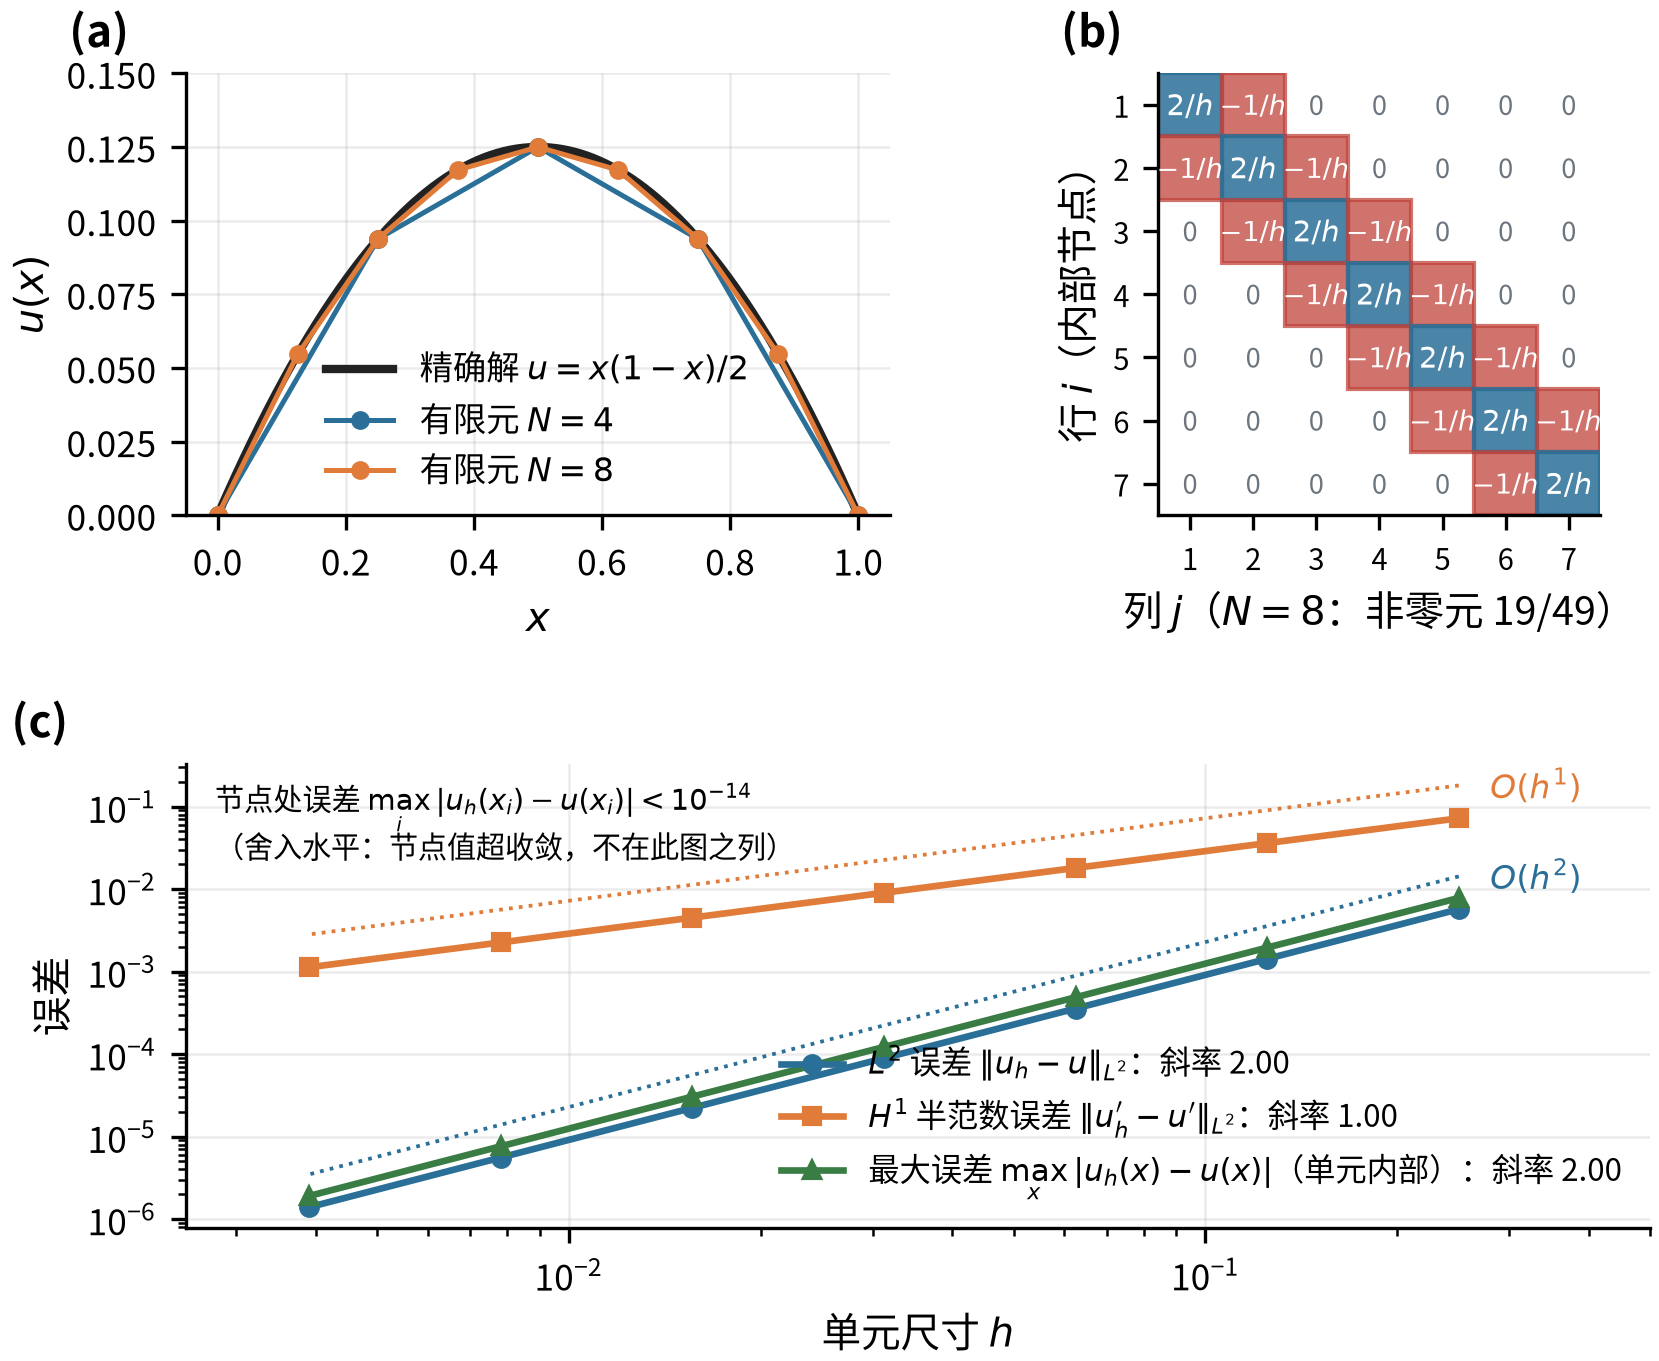
\includegraphics[width=0.95\textwidth]{figs_chap13/chap13_fig2.png}
\caption{一维有限元求解热传导问题$-u''=1$，$u(0)=u(1)=0$。(a) 有限元解（$N=4,8$）与解析解$u(x)=x(1-x)/2$的对比：节点值与解析解重合，误差只出现在单元内部。(b) 施加边界条件后的刚度矩阵$K$（$N=8$）的三对角结构——这源于帐篷函数的局部支撑性。(c) 网格细化时的收敛：$L^2$误差和单元内最大误差按$O(h^2)$下降（拟合斜率2.00），$H^1$半范数误差按$O(h)$下降（斜率1.00）；节点处的误差在$10^{-14}$以下（舍入水平），这是一维线性元的超收敛现象。}
\label{fig:chap13_fem}
\end{figure}

% ------------------------------------------------------------------------------------
\section{单元组装：从局部到整体}

上一节我们直接写出了整体刚度矩阵，这在一维均匀网格上没有问题；可一旦网格不规则、单元类型混杂，逐个推导 $K_{ij}$ 就无从下手了。实际计算中的做法分两步：先在每个小\textbf{单元}上计算\textbf{单元刚度矩阵}，再把所有单元刚度矩阵\textbf{组装}成整体刚度矩阵。这种“分而治之”的策略使有限元方法非常灵活——可以处理不规则网格、不同类型的单元混合等。

\subsection{单元刚度矩阵}

对于一维线性单元（两个节点），单元刚度矩阵是 $2 \times 2$ 的：

\begin{keyformula}[title=一维线性单元刚度矩阵]
\begin{equation}
K^e = \frac{1}{h}
\begin{pmatrix}
1 & -1 \\
-1 & 1
\end{pmatrix}
\end{equation}

行和列分别对应单元的左节点和右节点。
\end{keyformula}

\paragraph{推导}

设单元长度为 $h$，两端节点为 $x_L$ 和 $x_R$。

单元内的两个形函数：
\[
N_L(x) = \frac{x_R - x}{h}, \quad N_R(x) = \frac{x - x_L}{h}
\]

它们的导数：
\[
N_L' = -\frac{1}{h}, \quad N_R' = \frac{1}{h}
\]

单元刚度矩阵的元素：
\[
K^e_{LL} = \int_{x_L}^{x_R} (N_L')^2 dx = \frac{1}{h^2} \cdot h = \frac{1}{h}
\]
\[
K^e_{LR} = \int_{x_L}^{x_R} N_L' N_R' dx = -\frac{1}{h^2} \cdot h = -\frac{1}{h}
\]
\[
K^e_{RR} = \int_{x_L}^{x_R} (N_R')^2 dx = \frac{1}{h^2} \cdot h = \frac{1}{h}
\]

\subsection{组装过程}

组装的规则很简单：把每个单元刚度矩阵“放入”整体矩阵的对应位置，重叠处累加。

\begin{figure}[htbp]
\centering
\begin{tikzpicture}[scale=0.6]
    % 单元1矩阵（用数学矩阵表示，不用tikz框）
    \node[anchor=east] at (-2,6) {\small 单元1 (节点0-1):};
    \node at (0,6) {$\begin{pmatrix} \frac{1}{h} & -\frac{1}{h} \\[3pt] -\frac{1}{h} & \frac{1}{h} \end{pmatrix}$};

    % 箭头指向蓝色区域
    \draw[->, thick, blue!70] (1.8,6) -- (4.2,4.5);

    % 单元2矩阵
    \node[anchor=east] at (-2,2) {\small 单元2 (节点1-2):};
    \node at (0,2) {$\begin{pmatrix} \frac{1}{h} & -\frac{1}{h} \\[3pt] -\frac{1}{h} & \frac{1}{h} \end{pmatrix}$};

    % 箭头指向橙色区域
    \draw[->, thick, orange!80] (1.8,2) -- (5.2,2.5);

    % 整体矩阵框架
    \draw[thick] (4,0) grid (9,5);

    % 填充蓝色区域（单元1贡献：节点0,1）
    \fill[blue!25] (4,4) rectangle (5,5);
    \fill[blue!25] (5,4) rectangle (6,5);
    \fill[blue!25] (4,3) rectangle (5,4);
    \fill[blue!25] (5,3) rectangle (6,4);

    % 填充橙色区域（单元2贡献：节点1,2）
    \fill[orange!25] (5,3) rectangle (6,4);
    \fill[orange!25] (6,3) rectangle (7,4);
    \fill[orange!25] (5,2) rectangle (6,3);
    \fill[orange!25] (6,2) rectangle (7,3);

    % 重叠处（节点1的对角元）用红色标出
    \fill[red!40] (5,3) rectangle (6,4);
    \node[font=\footnotesize] at (5.5,3.5) {$\frac{2}{h}$};

    % 列标签（在矩阵上方）
    \foreach \i in {0,...,4} {
        \node[above, font=\scriptsize] at (4.5+\i,5.1) {\i};
    }
    % 行标签（在矩阵左侧）
    \foreach \i in {0,...,4} {
        \node[left, font=\scriptsize] at (3.9,4.5-\i) {\i};
    }

    % 整体矩阵标题
    \node[above] at (6.5,5.5) {\small 整体刚度矩阵 $K$};

    % 说明文字
    \node at (6.5,-0.8) {\small 重叠处累加：$\frac{1}{h} + \frac{1}{h} = \frac{2}{h}$};
\end{tikzpicture}
\caption{组装过程示意：单元矩阵放入整体矩阵对应位置，重叠处累加}
\end{figure}

\begin{physicalmeaning}
\textbf{组装的物理意义}：对角线元素 $K_{ii}$ 累加了所有与节点 $i$ 相连的单元贡献，是节点的“总刚度”；非对角线元素 $K_{ij}$ 只来自同时包含 $i$ 和 $j$ 的单元，是节点间的“耦合”。这就像一个弹簧网络：每个节点的总刚度是连接它的所有弹簧刚度之和。
\end{physicalmeaning}

% ------------------------------------------------------------------------------------
\section{边界条件处理}

到目前为止，边界条件是靠“只对内部节点列方程”悄悄处理掉的。这一节把这件事摆到明面上：边界条件到底怎么进入方程组，有几种进入方式，以及为什么其中一种会把第1章的乘子带回来。

\subsection{Dirichlet 边界条件（固定值）}

我们的例子中，$u(0) = u(1) = 0$ 是 Dirichlet 边界条件——边界上的值是固定的。

\paragraph{处理方法1：直接消去}

既然 $U_0 = U_4 = 0$ 是已知的，就从方程组中删去这两个未知量，只求解内部节点。

这就是我们上面手算例子用的方法。

\paragraph{处理方法2：大数法（罚函数）}

把对角线元素改成一个很大的数，对应的载荷也相应修改：

\[
K_{00} \leftarrow 10^{20}, \quad F_0 \leftarrow 10^{20} \times g_0
\]

其中 $g_0$ 是边界值。这样方程 $10^{20} U_0 = 10^{20} g_0$ 就强制 $U_0 \approx g_0$。

\textbf{优点}：不改变矩阵结构，易于编程

\textbf{缺点}：矩阵条件数变差

\subsection{Neumann 边界条件（给定导数）}

如果边界条件是 $u'(1) = q$（给定热流），这是 Neumann 边界条件。

Neumann 条件在弱形式中\textbf{自然满足}——它会贡献到载荷向量：
\[
F_n \leftarrow F_n + q
\]

\subsection{拉格朗日乘子法}

和第1章一样，我们也可以用拉格朗日乘子处理边界条件！

把边界条件 $u(0) = g$ 看作约束，引入乘子 $\lambda$：
\[
\mathcal{L}[u, \lambda] = J[u] + \lambda(u(0) - g)
\]

这导出一个\textbf{鞍点问题}：
\[
\begin{pmatrix}
K & B^\top \\
B & 0
\end{pmatrix}
\begin{pmatrix}
U \\
\lambda
\end{pmatrix}
=
\begin{pmatrix}
F \\
g
\end{pmatrix}
\]

\begin{physicalmeaning}
$\lambda$ 的物理意义是边界处的\textbf{法向通量}：在热传导里，$\lambda$ 是热流密度（W/m²）；在弹性力学里，$\lambda$ 是边界反力（N）。这与第5章力学中的约束力完全对应——边界条件本质上也是约束！
\end{physicalmeaning}
\review{第1章}{影子价格：$\lambda = -\dfrac{df^*}{d\epsilon}$。这里的 $\epsilon$ 是边界温度 $g$ 的微小改变，$f^*$ 是最小总势能。所以 $\lambda$ 度量“边界值抬高一点，总势能变多少”——量纲恰好是热流。}

% ------------------------------------------------------------------------------------
\section{误差分析与收敛性}

\subsection{误差的来源}

有限元解 $u_h$ 与精确解 $u$ 之间有误差。误差来自哪里？一方面是\textbf{离散化误差}——我们用有限维空间逼近了无限维空间；另一方面是\textbf{插值误差}——我们用分片多项式逼近了光滑函数。两者都随网格加密而减小，问题是减小得多快。

\subsection{误差估计}

对于线性形函数，误差有如下估计：

\begin{keytheorem}[title=有限元误差估计]
设 $u$ 是精确解，$u_h$ 是线性有限元解，$h$ 是网格步长。则：

\textbf{能量范数误差}：
\[
\|u' - u_h'\|_{L^2} \leq Ch \|u''\|_{L^2}
\]

\textbf{$L^2$ 范数误差}：
\[
\|u - u_h\|_{L^2} \leq Ch^2 \|u''\|_{L^2}
\]

其中 $C$ 是与 $h$ 无关的常数。
\end{keytheorem}

\paragraph{含义}

网格加密一倍（$h \to h/2$），导数误差减半，函数值误差减到 $\frac{1}{4}$。也就是说，线性元的收敛阶在能量范数下是 $O(h)$，在 $L^2$ 范数下是 $O(h^2)$；若用更高阶的多项式（如二次元、三次元），可以获得更高的收敛阶。

\subsection{数值验证}

让我们用不同的网格密度求解 $-u'' = 1$，验证收敛性：

\begin{center}
\begin{tabular}{c|c|c|c}
\toprule
单元数 $N$ & 步长 $h$ & 最大误差 & 误差比 \\
\midrule
4 & 0.25 & $7.8 \times 10^{-3}$ & -- \\
8 & 0.125 & $2.0 \times 10^{-3}$ & 3.9 \\
16 & 0.0625 & $4.9 \times 10^{-4}$ & 4.1 \\
32 & 0.03125 & $1.2 \times 10^{-4}$ & 4.1 \\
\bottomrule
\end{tabular}
\end{center}

每次加密一倍，误差减少到约 $\frac{1}{4}$——符合 $O(h^2)$ 的理论预测！
\clarify{表中的“最大误差”取在单元中点。前面说过一维线性元在节点处是精确的，所以误差全部来自节点之间的线性插值，中点误差恰好是 $h^2/8$（$h = 0.25$ 时为 $0.0078$）。}

% ------------------------------------------------------------------------------------
\section{二维问题简介}

\subsection{从一维到二维}

一维的思想可以自然推广到二维。

\textbf{二维 Poisson 方程}：
\[
-\nabla^2 u = -\left(\frac{\partial^2 u}{\partial x^2} + \frac{\partial^2 u}{\partial y^2}\right) = f \quad \text{in } \Omega
\]

\textbf{弱形式}：
\[
\int_\Omega \nabla u \cdot \nabla v \, dA = \int_\Omega fv \, dA
\]

\textbf{离散化}：把区域 $\Omega$ 剖分成三角形或四边形单元。

\begin{figure}[htbp]
\centering
\begin{tikzpicture}[scale=0.8]
    % 区域
    \draw[thick] (0,0) -- (4,0) -- (4,3) -- (0,3) -- cycle;
    
    % 三角形网格
    \foreach \x in {0,1,...,4} {
        \foreach \y in {0,1,2,3} {
            \fill (\x,\y) circle (1.5pt);
        }
    }
    
    % 画一些三角形
    \draw[gray] (0,0) -- (1,1) -- (0,1) -- cycle;
    \draw[gray] (0,0) -- (1,0) -- (1,1) -- cycle;
    \draw[gray] (1,0) -- (2,1) -- (1,1) -- cycle;
    \draw[gray] (1,0) -- (2,0) -- (2,1) -- cycle;
    \draw[gray] (2,0) -- (3,1) -- (2,1) -- cycle;
    \draw[gray] (2,0) -- (3,0) -- (3,1) -- cycle;
    \draw[gray] (3,0) -- (4,1) -- (3,1) -- cycle;
    \draw[gray] (3,0) -- (4,0) -- (4,1) -- cycle;
    
    \draw[gray] (0,1) -- (1,2) -- (0,2) -- cycle;
    \draw[gray] (0,1) -- (1,1) -- (1,2) -- cycle;
    \draw[gray] (1,1) -- (2,2) -- (1,2) -- cycle;
    \draw[gray] (1,1) -- (2,1) -- (2,2) -- cycle;
    \draw[gray] (2,1) -- (3,2) -- (2,2) -- cycle;
    \draw[gray] (2,1) -- (3,1) -- (3,2) -- cycle;
    \draw[gray] (3,1) -- (4,2) -- (3,2) -- cycle;
    \draw[gray] (3,1) -- (4,1) -- (4,2) -- cycle;
    
    \draw[gray] (0,2) -- (1,3) -- (0,3) -- cycle;
    \draw[gray] (0,2) -- (1,2) -- (1,3) -- cycle;
    \draw[gray] (1,2) -- (2,3) -- (1,3) -- cycle;
    \draw[gray] (1,2) -- (2,2) -- (2,3) -- cycle;
    \draw[gray] (2,2) -- (3,3) -- (2,3) -- cycle;
    \draw[gray] (2,2) -- (3,2) -- (3,3) -- cycle;
    \draw[gray] (3,2) -- (4,3) -- (3,3) -- cycle;
    \draw[gray] (3,2) -- (4,2) -- (4,3) -- cycle;
    
    % 标注
    \node at (2,-0.8) {三角形网格剖分};
\end{tikzpicture}
\caption{二维有限元：区域被剖分成三角形单元}
\end{figure}

\subsection{三角形单元}

最简单的二维单元是线性三角形单元。每个三角形有 3 个节点，单元内的近似解是：
\[
u_h(x, y) = U_1 N_1(x,y) + U_2 N_2(x,y) + U_3 N_3(x,y)
\]

其中 $N_i$ 是线性形函数，满足 $N_i(x_j, y_j) = \delta_{ij}$。

\paragraph{单元刚度矩阵}

三角形单元的刚度矩阵是 $3 \times 3$：
\[
K^e_{ij} = \int_{\text{三角形}} \nabla N_i \cdot \nabla N_j \, dA
\]

由于 $N_i$ 是线性函数，$\nabla N_i$ 是常向量，积分很容易计算。

\subsection{刚度矩阵的稀疏性}

二维问题的刚度矩阵仍然是稀疏的——只有相邻节点之间有耦合。

但稀疏结构更复杂：不再是三对角，而是\textbf{带状稀疏}矩阵。

\begin{figure}[htbp]
\centering
\begin{tikzpicture}[scale=0.08]
    % 画一个稀疏矩阵的样子
    \draw[gray] (0,0) rectangle (50,50);
    
    % 用随机点表示非零元素
    \foreach \i in {0,...,49} {
        \fill[blue] (\i,49-\i) circle (1);
        \pgfmathsetmacro{\jone}{int(\i+1)}
        \pgfmathsetmacro{\jtwo}{int(\i+2)}
        \pgfmathsetmacro{\jthree}{int(\i+5)}
        \pgfmathsetmacro{\jfour}{int(\i+6)}
        \ifnum\i<49
            \fill[blue!50] (\jone,49-\i) circle (0.8);
            \fill[blue!50] (\i,49-\jone) circle (0.8);
        \fi
        \ifnum\i<48
            \fill[blue!30] (\jtwo,49-\i) circle (0.6);
            \fill[blue!30] (\i,49-\jtwo) circle (0.6);
        \fi
        \ifnum\i<45
            \fill[blue!20] (\jthree,49-\i) circle (0.5);
            \fill[blue!20] (\i,49-\jthree) circle (0.5);
        \fi
    }
    
    \node at (25,-8) {\small 二维有限元的稀疏刚度矩阵};
\end{tikzpicture}
\end{figure}

% ------------------------------------------------------------------------------------
% ------------------------------------------------------------------------------------
\section{殊途同归：有限差分与有限元}

在继续深入之前，让我们回答一个常见问题：有限差分法（FDM）和有限元法（FEM）有什么区别？

\subsection{一维情况：完全等价}

考虑一维问题 $-u'' = f$，用 $N$ 个等距节点离散化。

\begin{figure}[htbp]
\centering
\begin{tikzpicture}[scale=1.2]
    % 左边：FDM
    \node[font=\bfseries] at (-3, 2) {有限差分 (FDM)};
    \draw[->] (-5, 0) -- (-1, 0) node[right] {$x$};
    \foreach \i in {0,1,2,3,4} {
        \fill (-5+\i, 0) circle (2pt);
        \node[below] at (-5+\i, -0.2) {\small $x_\i$};
    }
    % Taylor展开示意
    \draw[blue, thick, ->] (-3, 0.3) -- (-4, 0.3);
    \draw[blue, thick, ->] (-3, 0.3) -- (-2, 0.3);
    \node[blue, above] at (-3, 0.4) {\small Taylor展开};
    
    % 右边：FEM
    \node[font=\bfseries] at (3, 2) {有限元 (FEM)};
    \draw[->] (1, 0) -- (5, 0) node[right] {$x$};
    \foreach \i in {0,1,2,3,4} {
        \fill (1+\i, 0) circle (2pt);
    }
    % 形函数示意
    \draw[red, thick] (1,0) -- (2,0.8) -- (3,0);
    \draw[red, thick] (2,0) -- (3,0.8) -- (4,0);
    \node[red, above] at (3, 0.9) {\small 形函数};
\end{tikzpicture}
\caption{有限差分 vs 有限元的离散化方式}
\end{figure}

\vspace{0.3cm}
\noindent
\begin{minipage}[t]{0.48\textwidth}
\textbf{有限差分的推导}

出发点：Taylor展开近似导数
\[
-u''(x_i) \approx -\frac{u_{i+1} - 2u_i + u_{i-1}}{h^2}
\]

离散方程（第 $i$ 行）：
\[
\frac{-u_{i-1} + 2u_i - u_{i+1}}{h^2} = f_i
\]

系数：$\left[ -\frac{1}{h^2}, \; \frac{2}{h^2}, \; -\frac{1}{h^2} \right]$
\end{minipage}
\hfill
\begin{minipage}[t]{0.48\textwidth}
\textbf{有限元的推导}

出发点：弱形式 + 线性形函数
\[
K_{ij} = \int \phi_i' \phi_j' dx
\]

刚度矩阵（第 $i$ 行）：
\[
\frac{1}{h} [-1, \quad 2, \quad -1]
\]

方程：$\frac{-U_{i-1} + 2U_i - U_{i+1}}{h} = hf_i$
\end{minipage}

\vspace{0.5cm}
把FEM方程两边除以 $h$：
\[
\frac{-U_{i-1} + 2U_i - U_{i+1}}{h^2} = f_i
\]

\begin{insightbox}
在一维均匀网格上，线性有限元和中心差分给出\textbf{完全相同}的方程！

这不是巧合——两种方法从不同角度逼近了同一个物理问题。
\end{insightbox}



\subsection{二维情况：分道扬镳}

当问题升级到二维，两种方法开始展现本质区别。

\textbf{任务}：在圆形区域 $\Omega$ 上求解 $-\Delta u = f$。

\begin{figure}[htbp]
\centering
\begin{tikzpicture}[scale=1.8]
    % 左边：FDM
    \begin{scope}[xshift=-3cm]
        \node[font=\bfseries] at (0.5, 1.3) {有限差分};
        % 规则网格
        \draw[step=0.2, gray!30, thin] (0,0) grid (1.1,1.1);
        % 真实圆边界
        \draw[thick, red] (0,1) arc (90:0:1);
        % 锯齿逼近
        \draw[blue, thick]
            (0,1) -- (0.2,1) -- (0.2,0.8) --
            (0.4,0.8) -- (0.4,0.6) --
            (0.6,0.6) -- (0.6,0.4) --
            (0.8,0.4) -- (0.8,0.2) --
            (1.0,0.2) -- (1.0,0);
        % 五点差分模板
        \fill[blue] (0.6,0.4) circle (1pt);
        \foreach \dx/\dy in {0.2/0, -0.2/0, 0/0.2, 0/-0.2}{
            \draw[->, thick, blue!60] (0.6,0.4) -- +(\dx,\dy);
        }
        \node[red, font=\scriptsize] at (0.5, 1.15) {真实边界};
        \node[blue, font=\scriptsize] at (0.2, 0.5) {锯齿};
    \end{scope}
    
    % 右边：FEM
    \begin{scope}[xshift=1.5cm]
        \node[font=\bfseries] at (0.5, 1.3) {有限元};
        % 真实圆边界
        \draw[thick, red] (0,1) arc (90:0:1);
        % 三角剖分
        \coordinate (O) at (0,0);
        \coordinate (B) at (0,1);
        \coordinate (C) at (0.5,0.866);
        \coordinate (D) at (0.866,0.5);
        \coordinate (E) at (1,0);
        \coordinate (b) at (0,0.5);
        \coordinate (c) at (0.25,0.433);
        \coordinate (d) at (0.433,0.25);
        \coordinate (e) at (0.5,0);
        
        \draw[blue] (O) -- (b) -- (c) -- cycle;
        \draw[blue] (O) -- (c) -- (d) -- cycle;
        \draw[blue] (O) -- (d) -- (e) -- cycle;
        \draw[blue] (b) -- (B) -- (C) -- (c) -- cycle;
        \draw[blue] (c) -- (C) -- (D) -- (d) -- cycle;
        \draw[blue] (d) -- (D) -- (E) -- (e) -- cycle;
        
        % 边界节点
        \foreach \P in {B,C,D,E} {
            \fill[red] (\P) circle (1.5pt);
        }
        \node[blue, font=\scriptsize] at (0.5, 0.5) {三角形};
        \node[red, font=\scriptsize] at (0.7, 1.0) {节点在边界上};
    \end{scope}
\end{tikzpicture}
\caption{二维圆形区域的离散化：FDM用锯齿逼近边界，FEM可以精确贴合。}
\end{figure}

\begin{center}
\renewcommand{\arraystretch}{1.4}
\begin{tabular}{l|p{5cm}|p{5cm}}
\toprule
& \textbf{有限差分} & \textbf{有限元} \\
\midrule
网格类型 & 结构化（规则方格） & 非结构化（任意三角形） \\
边界处理 & 锯齿逼近，精度损失 & 节点直接在边界上 \\
复杂几何 & 困难（需要特殊处理） & 自然（只需网格生成） \\
实现难度 & 简单（数组索引） & 复杂（邻接关系） \\
适用场景 & 规则区域（图像、芯片） & 复杂几何（飞机、骨骼） \\
\bottomrule
\end{tabular}
\end{center}

\begin{physicalmeaning}
\textbf{为什么FEM统治了工程计算？}

现实世界的几何很少是规则的：飞机机翼是流线型的，人体骨骼是弯曲的，汽车车身是复杂曲面。

有限元的三角形/四面体网格可以\textbf{贴合任意几何形状}，这是它在工程中广泛应用的根本原因。

代价是：需要维护复杂的网格数据结构和邻接关系。
\end{physicalmeaning}

% ------------------------------------------------------------------------------------
\section{连续性的秘密}

\subsection{为什么要求连续？}

在前面的推导中，我们默默假设了 $u_h(x)$ 是连续的。但为什么？

\begin{figure}[htbp]
\centering
\begin{tikzpicture}[scale=1.2]
    % 上半部分：连续函数
    \begin{scope}[yshift=2cm]
        \draw[->] (0,0) -- (4,0) node[right] {$x$};
        \draw[->] (0,0) -- (0,1.5);
        \draw[blue, very thick] (0.5, 0.3) -- (2, 1.2) -- (3.5, 0.8);
        \node[blue] at (2, 1.5) {连续折线};
        \node[blue, align=center] at (5, 0.8) {导数有限 \\ 能量有限 $\checkmark$};
    \end{scope}
    
    % 下半部分：不连续函数
    \begin{scope}
        \draw[->] (0,0) -- (4,0) node[right] {$x$};
        \draw[->] (0,0) -- (0,1.5);
        \draw[red, very thick] (0.5, 0.3) -- (2, 1.2);
        \draw[red, very thick] (2, 0.4) -- (3.5, 0.8);
        \draw[red, dashed] (2, 0.4) -- (2, 1.2);
        \node[red] at (2.3, 0.8) {Jump!};
        \node[red, align=center] at (5, 0.8) {导数 $= \infty$ \\ 能量 $= \infty$ $\times$};
    \end{scope}
\end{tikzpicture}
\caption{连续性与能量的关系}
\end{figure}

\textbf{数学解释}：我们的弱形式包含梯度项 $\int |\nabla u|^2 dx$（能量）。如果 $u$ 在某点有跳跃（不连续），导数 $u'$ 在该点就变成 Dirac $\delta$ 函数（无穷大），于是能量 $\int (u')^2 dx = \int \delta^2 dx = \infty$。物理上，无穷大的能量是不允许的。

\begin{keyformula}[title=$C^0$ 连续性]
我们要求有限元解空间 $V_h \subset C^0(\Omega)$，即：

\textbf{函数值连续，但导数可以不连续}

换句话说：$u_h$ 可以“折”，但不能“断”。
\end{keyformula}

\subsection{线性单元如何保证连续？}

一个关键问题：我们只要求\textbf{节点值}相等，怎么能保证整条公共边上都连续？

\begin{figure}[htbp]
\centering
\begin{tikzpicture}[scale=1.5]
    % 两个三角形共享边
    \coordinate (N1) at (0,1);
    \coordinate (N2) at (0,-1);
    \coordinate (N3) at (-1.5, 0);
    \coordinate (N4) at (1.5, 0);
    
    \draw[fill=blue!10] (N1) -- (N2) -- (N3) -- cycle;
    \draw[fill=orange!10] (N1) -- (N2) -- (N4) -- cycle;
    
    % 共享边
    \draw[ultra thick, red] (N1) -- (N2);
    
    % 节点标注
    \node[above] at (N1) {$U_1$};
    \node[below] at (N2) {$U_2$};
    \node[left] at (N3) {$U_3$};
    \node[right] at (N4) {$U_4$};
    
    \node[blue] at (-0.7, 0) {单元 A};
    \node[orange] at (0.7, 0) {单元 B};
    
    % 边上的点
    \fill[black] (0, 0.3) circle (1.5pt) node[right] {$P$};
\end{tikzpicture}
\caption{两个三角形共享边 1-2}
\end{figure}

\textbf{几何证明}：

\begin{enumerate}
    \item 在三角形 A 内部，$u_h$ 是一个\textbf{平面}（线性函数）
    
    \item 这个平面在边 1-2 上截出一条\textbf{直线}
    
    \item 这条直线由两个端点值 $U_1$ 和 $U_2$ \textbf{唯一确定}（两点定一线！）
    
    \item 同样，三角形 B 在边 1-2 上也截出一条直线，也由 $U_1$ 和 $U_2$ 确定
    
    \item 两条直线端点相同 $\Rightarrow$ 两条直线重合！
\end{enumerate}

\begin{insightbox}
\textbf{线性单元连续性的关键}：两点确定一条直线。

只要共享节点的值相同，整条公共边就自动连续——就像\textbf{合页(Hinge)}一样严丝合缝。

这就是为什么线性单元只需要在顶点处设置自由度。
\end{insightbox}

\textbf{高阶单元怎么办？}

如果是二次单元，边上的函数是抛物线。两点定不了抛物线！

解决方案：在边的中点增加一个节点，三点定抛物线。

\begin{figure}[htbp]
\centering
\begin{tikzpicture}[scale=1.2]
    % 线性单元
    \begin{scope}
        \node[font=\bfseries] at (1, 1.8) {线性单元};
        \draw[thick] (0,0) -- (2,0) -- (1,1.5) -- cycle;
        \fill[blue] (0,0) circle (3pt);
        \fill[blue] (2,0) circle (3pt);
        \fill[blue] (1,1.5) circle (3pt);
        \node[below] at (1, -0.3) {3个节点};
    \end{scope}
    
    % 二次单元
    \begin{scope}[xshift=5cm]
        \node[font=\bfseries] at (1, 1.8) {二次单元};
        \draw[thick] (0,0) -- (2,0) -- (1,1.5) -- cycle;
        % 顶点
        \fill[blue] (0,0) circle (3pt);
        \fill[blue] (2,0) circle (3pt);
        \fill[blue] (1,1.5) circle (3pt);
        % 边中点
        \fill[red] (1,0) circle (3pt);
        \fill[red] (1.5,0.75) circle (3pt);
        \fill[red] (0.5,0.75) circle (3pt);
        \node[below] at (1, -0.3) {6个节点};
    \end{scope}
\end{tikzpicture}
\caption{线性单元（3节点）vs 二次单元（6节点）}
\end{figure}

\subsection{一维二次单元详解}

为了理解高阶单元，让我们先看最简单的情况：一维二次单元。

\begin{figure}[htbp]
\centering
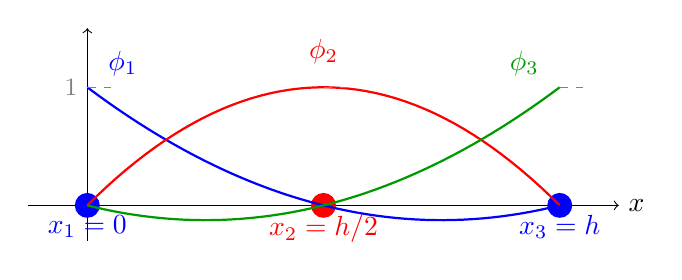
\begin{tikzpicture}[scale=1.5]
    % 坐标轴
    \draw[->] (-0.5, 0) -- (4.5, 0) node[right] {$x$};
    \draw[->] (0, -0.3) -- (0, 1.5);
    
    % 三个节点
    \fill[blue] (0, 0) circle (3pt) node[below] {$x_1 = 0$};
    \fill[red] (2, 0) circle (3pt) node[below] {$x_2 = h/2$};
    \fill[blue] (4, 0) circle (3pt) node[below] {$x_3 = h$};
    
    % 三个形函数
    % φ_1: 在x_1=1, 其他=0
    \draw[blue, thick, domain=0:4, samples=50] plot (\x, {((\x-2)*(\x-4))/((-2)*(-4))});
    \node[blue] at (0.3, 1.2) {$\phi_1$};
    
    % φ_2: 在x_2=1, 其他=0
    \draw[red, thick, domain=0:4, samples=50] plot (\x, {((\x-0)*(\x-4))/((2-0)*(2-4))});
    \node[red] at (2, 1.3) {$\phi_2$};
    
    % φ_3: 在x_3=1, 其他=0
    \draw[green!60!black, thick, domain=0:4, samples=50] plot (\x, {((\x-0)*(\x-2))/((4-0)*(4-2))});
    \node[green!60!black] at (3.7, 1.2) {$\phi_3$};
    
    % 高度标记
    \draw[dashed, gray] (0, 1) -- (0.2, 1);
    \node[left, gray] at (0, 1) {\small 1};
    \draw[dashed, gray] (2, 1) -- (2.2, 1);
    \draw[dashed, gray] (4, 1) -- (4.2, 1);
\end{tikzpicture}
\caption{一维二次单元的三个形函数：都是抛物线！}
\end{figure}

\textbf{二次形函数的公式}

用拉格朗日插值构造（三点定抛物线）：

\begin{align}
\phi_1(x) &= \frac{(x - x_2)(x - x_3)}{(x_1 - x_2)(x_1 - x_3)} = \frac{(x - h/2)(x - h)}{(0 - h/2)(0 - h)} = \frac{2(x - h/2)(x - h)}{h^2} \\[5pt]
\phi_2(x) &= \frac{(x - x_1)(x - x_3)}{(x_2 - x_1)(x_2 - x_3)} = \frac{(x - 0)(x - h)}{(h/2)(- h/2)} = -\frac{4x(x - h)}{h^2} \\[5pt]
\phi_3(x) &= \frac{(x - x_1)(x - x_2)}{(x_3 - x_1)(x_3 - x_2)} = \frac{(x - 0)(x - h/2)}{(h)(h/2)} = \frac{2x(x - h/2)}{h^2}
\end{align}

可以验证：$\phi_i(x_j) = \delta_{ij}$（在自己的节点上等于1，其他节点上等于0）。

\begin{example}[二次单元的刚度矩阵]
计算一维二次单元的刚度矩阵 $K_{ij} = \int_0^h \phi_i'(x) \phi_j'(x) dx$。

\textbf{Step 1: 求导}

先对形函数求导（注意这次导数不再是常数了！）：
\begin{align}
\phi_1'(x) &= \frac{2(2x - 3h/2)}{h^2} = \frac{4x - 3h}{h^2} \\[3pt]
\phi_2'(x) &= \frac{-4(2x - h)}{h^2} = \frac{-8x + 4h}{h^2} \\[3pt]
\phi_3'(x) &= \frac{2(2x - h/2)}{h^2} = \frac{4x - h}{h^2}
\end{align}

\textbf{Step 2: 计算 $K_{11}$}
\begin{align}
K_{11} &= \int_0^h (\phi_1')^2 dx = \int_0^h \frac{(4x - 3h)^2}{h^4} dx \\
&= \frac{1}{h^4} \int_0^h (16x^2 - 24hx + 9h^2) dx \\
&= \frac{1}{h^4} \left[ \frac{16x^3}{3} - 12hx^2 + 9h^2 x \right]_0^h \\
&= \frac{1}{h^4} \left( \frac{16h^3}{3} - 12h^3 + 9h^3 \right) = \frac{1}{h^4} \cdot \frac{7h^3}{3} = \boxed{\frac{7}{3h}}
\end{align}

\textbf{Step 3: 计算 $K_{12}$}
\begin{align}
K_{12} &= \int_0^h \phi_1' \phi_2' dx = \int_0^h \frac{(4x - 3h)(-8x + 4h)}{h^4} dx \\
&= \frac{1}{h^4} \int_0^h (-32x^2 + 40hx - 12h^2) dx \\
&= \frac{1}{h^4} \left[ -\frac{32x^3}{3} + 20hx^2 - 12h^2 x \right]_0^h \\
&= \frac{1}{h^4} \left( -\frac{32h^3}{3} + 20h^3 - 12h^3 \right) = \frac{1}{h^4} \cdot \left(-\frac{8h^3}{3}\right) = \boxed{-\frac{8}{3h}}
\end{align}

\textbf{完整的刚度矩阵}（类似计算其他元素后）：
\begin{equation}
K^{(e)} = \frac{1}{3h} \begin{pmatrix}
7 & -8 & 1 \\
-8 & 16 & -8 \\
1 & -8 & 7
\end{pmatrix}
\end{equation}
\end{example}

\begin{physicalmeaning}
对比线性单元和二次单元的刚度矩阵：

\vspace{0.3cm}
\begin{minipage}[t]{0.45\textwidth}
\centering
\textbf{线性单元}（2节点）
\[
K^{(e)} = \frac{1}{h} \begin{pmatrix}
1 & -1 \\
-1 & 1
\end{pmatrix}
\]
只有相邻节点耦合
\end{minipage}
\hfill
\begin{minipage}[t]{0.45\textwidth}
\centering
\textbf{二次单元}（3节点）
\[
K^{(e)} = \frac{1}{3h} \begin{pmatrix}
7 & -8 & 1 \\
-8 & 16 & -8 \\
1 & -8 & 7
\end{pmatrix}
\]
三个节点都有耦合！
\end{minipage}

\vspace{0.3cm}
注意二次单元中 $K_{13} = \frac{1}{3h} \neq 0$：端点1和端点3虽然不相邻，但通过中间的抛物线“感受”到彼此！
\end{physicalmeaning}

\begin{example}[精度提升的威力]
用二次单元求解 $-u'' = 1$，$u(0) = u(1) = 0$。

只用\textbf{2个二次单元}（5个节点：$x = 0, 0.25, 0.5, 0.75, 1$）：

\begin{center}
\begin{tabular}{c|c|c|c}
\toprule
$x$ & 数值解 $U$ & 精确解 $u = \frac{x(1-x)}{2}$ & 误差 \\
\midrule
0 & 0 & 0 & 0 \\
0.25 & 0.09375 & 0.09375 & 0 \\
0.5 & 0.125 & 0.125 & 0 \\
0.75 & 0.09375 & 0.09375 & 0 \\
1 & 0 & 0 & 0 \\
\bottomrule
\end{tabular}
\end{center}

误差为\textbf{零}！因为精确解是二次多项式，而二次单元可以精确表示二次多项式。

这叫做\textbf{多项式精确性}：$p$阶单元可以精确表示$p$阶及以下的多项式。
\end{example}

\begin{insightbox}
\textbf{高阶单元的代价与收益}：代价是每个单元的节点数增加（线性 3 个 $\to$ 二次 6 个），单元刚度矩阵更大、计算量增加，形函数也更复杂、需要数值积分。收益是相同网格下精度大幅提高，收敛速度从 $O(h^2)$ 提高到 $O(h^3)$，对于光滑解常常“事半功倍”。工程中的经验法则：对于光滑问题，用少量高阶单元往往比大量低阶单元更高效！
\end{insightbox}
% ------------------------------------------------------------------------------------
\section{全局视角：帐篷函数的叠加}

\subsection{从单元思维到全局思维}

前面我们一直从“拼装单元”的角度理解有限元。现在换个视角：

与其说是“把单元拼起来”，不如说是“把全局基函数叠加起来”。

\begin{figure}[htbp]
\centering
\begin{tikzpicture}[scale=0.7, x={(1cm,0cm)}, y={(0.5cm,0.4cm)}, z={(0cm,1cm)}]
    % 中心点
    \coordinate (C) at (0,0,0);
    \coordinate (Top) at (0,0,2.5);
    
    % 周围一圈点 (六边形)
    \foreach \i in {0, 60, ..., 300} {
        \coordinate (P\i) at ({2.5*cos(\i)}, {2.5*sin(\i)}, 0);
        \draw[gray] (C) -- (P\i);
        \draw[blue, thick] (Top) -- (P\i);
    }
    % 连外圈
    \draw[gray] (P0)--(P60)--(P120)--(P180)--(P240)--(P300)--cycle;
    
    % 填充几个面
    \fill[blue!20, opacity=0.5] (P0)--(Top)--(P60)--cycle;
    \fill[blue!30, opacity=0.5] (P60)--(Top)--(P120)--cycle;
    \fill[blue!15, opacity=0.5] (P120)--(Top)--(P180)--cycle;
    
    \node[above, red, font=\bfseries] at (Top) {$\Phi_i = 1$};
    \node[below] at (C) {节点 $i$};
    \node[gray] at (3, 0, 0) {$\Phi_i = 0$};
\end{tikzpicture}
\caption{全局形函数 $\Phi_i$：一个以节点 $i$ 为顶点的“帐篷”}
\end{figure}

全局形函数 $\Phi_i$ 在节点 $i$ 处取值为 1，在所有邻居节点处取值为 0，在其他地方也是 0（局部支撑），形状像一个多面体的“帐篷”或“金字塔”。有限元解可以写成：
\begin{equation}
u_h(x) = \sum_{i=1}^{N} U_i \Phi_i(x)
\end{equation}

这就是 $N$ 个帐篷高低错落地叠加在一起！

\begin{physicalmeaning}
\textbf{连续性的本质}：

每个全局基函数 $\Phi_i$ 本身都是连续的（帐篷布没有破洞）。

连续函数的线性组合还是连续函数。

所以 $u_h = \sum U_i \Phi_i$ 必然是连续的！

“节点共享”的本质，是我们定义了\textbf{跨越多个单元的全局基函数}。
\end{physicalmeaning}

\subsection{稀疏性的来源}

刚度矩阵为什么是稀疏的？

\begin{equation}
K_{ij} = \int_\Omega \nabla\Phi_i \cdot \nabla\Phi_j \, dx
\end{equation}

关键观察：$\Phi_i$ 和 $\Phi_j$ 只在它们的支撑区域重叠时，积分才非零！

\begin{figure}[htbp]
\centering
\begin{tikzpicture}[scale=1.5]
    % 中心点 i
    \coordinate (Ni) at (0,0);
    
    % i 的影响范围
    \fill[red!15] (1,0) -- (0.5, 0.866) -- (-0.5, 0.866) -- (-1,0) -- (-0.5, -0.866) -- (0.5, -0.866) -- cycle;
    
    % 画中心点
    \fill[red] (Ni) circle (2.5pt);
    \node[red, below=3pt] at (Ni) {$U_i$};
    
    % 邻居节点
    \foreach \angle/\idx in {0/1, 60/2, 120/3, 180/4, 240/5, 300/6} {
        \coordinate (Nj\idx) at (\angle:1);
        \draw[thick, gray] (Ni) -- (Nj\idx);
        \fill[blue] (Nj\idx) circle (2pt);
    }
    
    % 远处的点
    \coordinate (Nk) at (1.8, 0.8);
    \fill[black!50] (Nk) circle (2pt);
    \node[right, font=\small] at (Nk) {$U_k$（非邻居）};
    
    \draw[dashed, gray] (Ni) -- (Nk);
    \node[font=\scriptsize, gray] at (1.2, 0.5) {$K_{ik} = 0$};
\end{tikzpicture}
\caption{节点 $i$ 只与直接相邻的节点耦合}
\end{figure}

如果节点 $i$ 和 $j$ 直接相邻（有边相连），$\Phi_i$ 和 $\Phi_j$ 重叠，$K_{ij} \neq 0$；如果节点 $i$ 和 $j$ 不相邻，$\Phi_i$ 和 $\Phi_j$ 不重叠，$K_{ij} = 0$。

\begin{insightbox}
\textbf{稀疏性的物理意义}：

即使网格有100万个节点，每个节点也只与周围约6-8个邻居耦合。

刚度矩阵的每一行只有约7个非零元素（自己 + 6个邻居）。

这就是为什么我们能求解大规模有限元问题——矩阵虽大，但几乎全是零！
\end{insightbox}

% ------------------------------------------------------------------------------------
\section{与优化的联系}

让我们从拉格朗日乘子的角度重新审视有限元。

\subsection{有限元 = 能量最小化}

回顾一下有限元的推导路径：

\begin{center}
\begin{tikzpicture}[node distance=3.25cm, auto,
    block/.style={rectangle, draw, fill=blue!10, text width=2.5cm, text centered, rounded corners, minimum height=1.2cm, font=\small}]
    \node[block] (pde) {PDE\\[2pt]$-\Delta u = f$};
    \node[block, right of=pde] (var) {变分问题\\[2pt]$\min J[u]$};
    \node[block, right of=var] (weak) {弱形式\\[2pt]$\int \nabla u \cdot \nabla v = \int fv$};
    \node[block, right of=weak] (lin) {线性方程\\[2pt]$KU = F$};

    \draw[->, thick] (pde) -- (var);
    \draw[->, thick] (var) -- (weak);
    \draw[->, thick] (weak) -- (lin);
\end{tikzpicture}
\end{center}

有限元方程 $KU = F$ 其实是以下优化问题的\textbf{一阶最优性条件}：

\begin{equation}
\min_U \quad J(U) = \frac{1}{2}U^\top K U - F^\top U
\end{equation}

求导：$\nabla_U J = KU - F = 0 \quad \Rightarrow \quad KU = F$

\begin{physicalmeaning}
$J(U) = \frac{1}{2}U^\top KU - F^\top U$ 的物理意义：$\frac{1}{2}U^\top KU$ 是系统的内部能量（弹性势能、热能等），$F^\top U$ 是外力做的功，两者之差 $J(U)$ 就是总势能。\textbf{有限元求解的本质}是找到使总势能最小的状态，这与自然界的规律一致——系统总是趋向于能量最低的平衡态！
\end{physicalmeaning}

\subsection{约束处理的统一视角}

现在，边界条件可以被理解为\textbf{约束}：

\begin{center}
\renewcommand{\arraystretch}{1.5}
\begin{tabular}{c|c|c}
\toprule
\textbf{优化概念} & \textbf{有限元对应} & \textbf{物理意义} \\
\midrule
决策变量 $U$ & 节点值 $U_i$ & 温度/位移 \\
目标函数 $J(U)$ & $\frac{1}{2}U^\top KU - F^\top U$ & 总势能 \\
等式约束 $CU = g$ & Dirichlet 边界条件 & 固定边界 \\
拉格朗日乘子 $\lambda$ & 边界反力/热流 & 约束力 \\
\bottomrule
\end{tabular}
\end{center}

带边界条件的有限元问题：
\begin{align}
\min_U \quad & \frac{1}{2}U^\top K U - F^\top U \\
\text{s.t.} \quad & U_i = g_i \quad \text{（边界节点）}
\end{align}

拉格朗日函数：
\begin{equation}
\mathcal{L}(U, \lambda) = \frac{1}{2}U^\top K U - F^\top U + \sum_{i \in \text{边界}} \lambda_i (U_i - g_i)
\end{equation}

\begin{keytheorem}[title=乘子的物理意义]
有限元中的拉格朗日乘子 $\lambda_i$ = 边界节点 $i$ 处的\textbf{反力}（或热流）。

它告诉我们：\textbf{为了维持边界条件，需要施加多大的外力}。
\end{keytheorem}

\begin{example}[悬臂梁]
考虑一端固定的悬臂梁，固定端位移为零：$U_1 = 0$。

拉格朗日乘子 $\lambda_1$ 就是固定端的支反力——墙壁对梁的作用力。

如果放松约束（允许 $U_1$ 有微小位移 $\delta U_1$），最小总势能会改变 $-\lambda_1\, \delta U_1$——这正是第1章的约定 $dJ^*/dg = -\lambda$：乘子就是影子价格。
\end{example}
\review{第5章}{在第5章，乘子 $\lambda$ 给出约束力（绳子的张力、斜面的支持力）。这里的 $\lambda_1$ 是墙对梁的支反力——同一个东西，只是从“连续体”换成了“离散节点”。}

% ------------------------------------------------------------------------------------
\section{打破传统：间断有限元初探}

前面我们花了很大功夫保证有限元解的连续性。但有没有可能\textbf{故意让它不连续}？

\subsection{一个大胆的想法}

传统有限元的“痛点”都来自节点共享：必须维护复杂的节点共享关系，网格生成困难（要保证相邻单元节点对齐），也难以并行化（单元之间有耦合）。\textbf{新思路}是让每个单元拥有\textbf{独立的节点}，然后用\textbf{约束}把它们“缝合”起来！

\begin{figure}[htbp]
\centering
\begin{tikzpicture}[scale=1.5]
    % 左边：传统FEM
    \begin{scope}
        \node[font=\bfseries] at (0.75, 1.5) {传统 FEM};
        \coordinate (A) at (0,0);
        \coordinate (B) at (1.5,0);
        \coordinate (C) at (0.75, 1.2);
        \coordinate (D) at (2.25, 1.2);
        
        \draw[thick, fill=blue!10] (A)--(B)--(C)--cycle;
        \draw[thick, fill=orange!10] (B)--(D)--(C)--cycle;
        
        \fill[red] (B) circle (2pt) node[below]{$U_2$};
        \fill[red] (C) circle (2pt) node[above]{$U_3$};
        
        \node[align=center, font=\scriptsize] at (0.75, -0.5) {共享节点\\$U_2, U_3$ 只有一份};
    \end{scope}
    
    % 右边：间断FEM
    \begin{scope}[xshift=4cm]
        \node[font=\bfseries] at (0.75, 1.5) {间断 FEM};
        % 左单元
        \coordinate (A) at (0,0);
        \coordinate (B1) at (1.4,0);
        \coordinate (C1) at (0.65, 1.2);
        \draw[thick, fill=blue!10] (A)--(B1)--(C1)--cycle;
        
        % 右单元（稍微拉开）
        \coordinate (B2) at (1.6,0);
        \coordinate (C2) at (0.85, 1.2);
        \coordinate (D) at (2.35, 1.2);
        \draw[thick, fill=orange!10] (B2)--(D)--(C2)--cycle;
        
        \fill[blue] (B1) circle (2pt) node[below left=-2pt, font=\scriptsize]{$U_2^{(1)}$};
        \fill[blue] (C1) circle (2pt) node[above left=-2pt, font=\scriptsize]{$U_3^{(1)}$};
        \fill[orange] (B2) circle (2pt) node[below right=-2pt, font=\scriptsize]{$U_2^{(2)}$};
        \fill[orange] (C2) circle (2pt) node[above right=-2pt, font=\scriptsize]{$U_3^{(2)}$};
        
        \draw[<->, dashed, red] (B1)--(B2);
        \node[red, font=\scriptsize] at (1.5, -0.3) {Gap};
        
        \node[align=center, font=\scriptsize] at (0.75, -0.5) {独立节点\\需要约束缝合};
    \end{scope}
\end{tikzpicture}
\caption{传统FEM（共享节点）vs 间断FEM（独立节点）}
\end{figure}

\subsection{变量倍增与约束方程}

\textbf{变量变化}：传统做法的未知量是 $U = [U_1, U_2, U_3, U_4]$，共 4 个；间断做法把共享节点拆开，未知量变成 $U = [U_1^{(1)}, U_2^{(1)}, U_3^{(1)}, U_2^{(2)}, U_3^{(2)}, U_4^{(2)}]$，共 6 个。

\textbf{新增约束}（缝合条件）：
\begin{equation}
U_2^{(1)} = U_2^{(2)}, \quad U_3^{(1)} = U_3^{(2)}
\end{equation}

写成矩阵形式：$CU = 0$，其中
\begin{equation}
C = \begin{bmatrix}
0 & 1 & 0 & -1 & 0 & 0 \\
0 & 0 & 1 & 0 & -1 & 0
\end{bmatrix}
\end{equation}

\subsection{用拉格朗日乘子缝合}

新的优化问题：
\begin{align}
\min_U \quad & \frac{1}{2}U^\top K_{block} U - F^\top U \\
\text{s.t.} \quad & CU = 0 \quad \text{（缝合条件）}
\end{align}

其中 $K_{block}$ 是\textbf{块对角矩阵}：
\begin{equation}
K_{block} = \begin{bmatrix}
K^{(1)} & 0 \\
0 & K^{(2)}
\end{bmatrix}
\end{equation}

拉格朗日函数：
\begin{equation}
\mathcal{L}(U, \lambda) = \frac{1}{2}U^\top K_{block} U - F^\top U + \lambda^\top (CU)
\end{equation}

\begin{physicalmeaning}
乘子 $\lambda$ 的物理意义：\textbf{界面力}（interface flux）。

它是维持单元之间连续性的“胶水力”——强制两边位移相等的约束力。

这与传统FEM中隐式存在的单元间作用力是一样的，只不过现在被显式地表示出来了！
\end{physicalmeaning}

\subsection{块对角结构的威力}

间断有限元的最大优势：$K_{block}$ 是块对角的！

\begin{equation}
K_{block}^{-1} = \begin{bmatrix}
(K^{(1)})^{-1} & 0 \\
0 & (K^{(2)})^{-1}
\end{bmatrix}
\end{equation}

\textbf{这意味着}：每个单元可以\textbf{独立求解}！
\clarify{“每个单元独立求解”有个前提：界面力 $\lambda$ 已知。$\lambda$ 本身要靠界面方程解出——这正是本章扩展阅读里 Schur 补与区域分解的思路。}

\begin{center}
\renewcommand{\arraystretch}{1.4}
\begin{tabular}{l|c|c}
\toprule
& \textbf{传统 FEM} & \textbf{间断 FEM} \\
\midrule
刚度矩阵结构 & 稀疏但耦合 & 块对角 \\
单元独立求解 & 不可能 & 可以！ \\
并行化 & 困难 & 天然并行 \\
GPU 加速 & 有限 & 极度友好 \\
\bottomrule
\end{tabular}
\end{center}

\begin{insightbox}
\textbf{为什么这很重要？}

现代 GPU 有数千个核心，但它们最擅长的是做\textbf{相同的独立计算}。

间断有限元把一个大问题分解成了百万个 $3 \times 3$（或 $4 \times 4$）的小问题，每个核心解一个——这正是 GPU 的最爱！

这就是为什么间断 Galerkin (DG) 方法在计算流体力学等领域越来越流行。
\end{insightbox}

\subsection{罚函数方法：软约束}

直接处理带约束的鞍点问题比较复杂。一个常用技巧是\textbf{罚函数}：

不强制 $U^{(1)} = U^{(2)}$，而是惩罚它们的差距：
\begin{equation}
J_\rho(U) = \frac{1}{2}U^\top K_{block} U - F^\top U + \frac{\rho}{2}\|CU\|^2
\end{equation}

其中 $\rho$ 是罚参数（很大的正数）——记号与第1章“视角三：罚函数”一致。

\begin{figure}[htbp]
\centering
\begin{tikzpicture}[scale=0.9]
    % 弱罚
    \begin{scope}
        \node[font=\bfseries] at (1.5, 1.8) {弱罚（$\rho$ 小）};
        \draw[fill=blue!20, thick] (0,0) rectangle (2,1);
        \draw[fill=blue!20, thick] (2.5,0) rectangle (4.5,1);
        \draw[decorate, decoration={coil,aspect=0.5,segment length=3mm,amplitude=3mm}, thick, red] (2,0.5) -- (2.5,0.5);
        \node[red, font=\small] at (2.25, 1.3) {Gap 大};
        \node at (1, 0.5) {单元1};
        \node at (3.5, 0.5) {单元2};
    \end{scope}
    
    % 强罚
    \begin{scope}[xshift=6cm]
        \node[font=\bfseries] at (1.5, 1.8) {强罚（$\rho \to \infty$）};
        \draw[fill=blue!20, thick] (0,0) rectangle (2.1,1);
        \draw[fill=blue!20, thick] (2.2,0) rectangle (4.3,1);
        \draw[decorate, decoration={coil,aspect=0.3,segment length=1mm,amplitude=2mm}, thick, red] (2.1,0.5) -- (2.2,0.5);
        \node[red, font=\small] at (2.15, 1.3) {Gap $\approx 0$};
        \node at (1, 0.5) {单元1};
        \node at (3.25, 0.5) {单元2};
    \end{scope}
\end{tikzpicture}
\caption{罚函数就像在断口处装了一个弹簧}
\end{figure}

当 $\rho \to \infty$ 时，任何微小的 Gap 都会产生巨大的惩罚，系统被迫让 $CU \to 0$，于是恢复到传统有限元的连续解。

\begin{physicalmeaning}
罚函数的物理图像：在断口处装一个\textbf{刚度为 $\rho$ 的弹簧}。$\rho$ 小，弹簧软，拉不住，Gap 大；$\rho$ 大，弹簧硬，瞬间把两端吸在一起。这与深度学习中的正则化项异曲同工！
\[
\text{Loss} = \text{Data\_Fidelity} + \rho \cdot \text{Regularization}
\]

这个思想也激励了我们探索物理信息神经网络(PINN)。
\end{physicalmeaning}

% ------------------------------------------------------------------------------------
% ------------------------------------------------------------------------------------
\section{本章小结}

\begin{enumerate}
    \item \textbf{核心思想}：有限元方法把无限维的变分问题转化为有限维的线性方程组 $KU = F$。
    
    \item \textbf{与有限差分的关系}：一维等价，二维开始分化；FEM 的优势在于处理复杂几何。
    
    \item \textbf{连续性}：$C^0$ 连续性保证能量有限；线性单元靠“两点定一线”自动满足连续性。
    
    \item \textbf{全局视角}：有限元解是全局“帐篷”基函数的线性叠加。
    
    \item \textbf{稀疏性}：基函数的局部支撑性导致刚度矩阵稀疏。
    
    \item \textbf{优化视角}：有限元 $\Leftrightarrow$ 能量最小化 $\Leftrightarrow$ 带约束的 QP 问题。
    
    \item \textbf{间断有限元}：放弃强制连续性，用约束/罚函数缝合，获得天然并行性。
\end{enumerate}

\begin{unification}[title=有限元：优化视角的大统一]
\begin{center}
\begin{tabular}{lll}
\toprule
\textbf{优化概念} & \textbf{有限元对应} & \textbf{物理意义} \\
\midrule
决策变量 & 节点值 $U_i$ & 物理量（温度/位移） \\
目标函数 & $\frac{1}{2}U^\top KU - F^\top U$ & 总势能 \\
等式约束 & Dirichlet 边界条件 & 固定边界 \\
拉格朗日乘子 & 边界反力 & 约束力 \\
罚函数 & 界面耦合项 & 虚拟弹簧 \\
\bottomrule
\end{tabular}
\end{center}

有限元不是孤立的数值技术，它是\textbf{变分原理}和\textbf{约束优化}在工程中的自然统一！

从第1章的拉格朗日乘子，到这里的有限元，$\lambda$ 始终扮演着“约束力”的角色。
\end{unification}

\begin{physicalmeaning}
\textbf{$\lambda$ 在本章的意义}：边界条件是约束，$\lambda$ 是“把边界钉住”所需的力——热传导里是边界热流，弹性力学里是支反力，间断元里是单元之间的界面力。它仍然是影子价格：$\lambda_i = -\partial J^*/\partial g_i$，边界值放松一点，最小总势能就改变 $\lambda_i$ 那么多。

回头看：第1章的 $\lambda$ 是影子价格，第5章的 $\lambda$ 是约束力，本章把两者接在了一起——约束力就是能量对约束的敏感度。往前看：第6章机器人的接触力，以及第14章 PINN 把 PDE 当作软约束写进损失函数，用的都是同一个 $\lambda$。
\end{physicalmeaning}


% ------------------------------------------------------------------------------------
\section{习题}

\paragraph{计算题}
\begin{enumerate}
    \item 用 2 个线性单元求解 $-u'' = 1$，$u(0) = u(1) = 0$。
    \begin{enumerate}
        \item 写出刚度矩阵 $K$ 和载荷向量 $F$
        \item 求解线性方程组，得到节点值 $U_1$
        \item 与精确解 $u(0.5) = 0.125$ 比较
    \end{enumerate}
    
    \item 用 4 个线性单元求解 $-u'' = \sin(\pi x)$，$u(0) = u(1) = 0$。
    \begin{enumerate}
        \item 计算载荷向量（需要积分 $\int \sin(\pi x) \phi_i dx$）
        \item 求解节点值
        \item 与精确解 $u(x) = \frac{\sin(\pi x)}{\pi^2}$ 比较
    \end{enumerate}
    
    \item 考虑非齐次边界条件：$-u'' = 0$，$u(0) = 0$，$u(1) = 1$。
    \begin{enumerate}
        \item 用 3 个单元建立有限元方程
        \item 用直接消去法处理边界条件
        \item 求解并验证结果是直线 $u(x) = x$
    \end{enumerate}
\end{enumerate}

\paragraph{证明题}
\begin{enumerate}
    \setcounter{enumi}{3}
    \item 证明刚度矩阵 $K$ 是对称的：$K_{ij} = K_{ji}$。
    
    \item 证明刚度矩阵 $K$ 是半正定的：$U^\top K U \geq 0$ 对所有 $U$ 成立。
    
    \item 证明有限元解 $u_h$ 是精确解 $u$ 在有限元空间中的“最佳逼近”：
    \[
    \int_0^1 (u_h' - u')^2 dx \leq \int_0^1 (v_h' - u')^2 dx \quad \forall v_h \in V_h
    \]
    （提示：这叫做 Galerkin 正交性）
\end{enumerate}

\paragraph{编程题}
\begin{enumerate}
    \setcounter{enumi}{6}
    \item 实现一维线性有限元：
    \begin{enumerate}
        \item 输入：区间 $[0, 1]$，单元数 $N$，源项 $f(x)$，边界值
        \item 输出：节点值向量 $U$
        \item 测试：$-u'' = 1$，$u(0) = u(1) = 0$
    \end{enumerate}
    
    \item 做收敛性实验：
    \begin{enumerate}
        \item 用 $N = 4, 8, 16, 32, 64$ 个单元求解
        \item 计算误差 $\|u - u_h\|_{L^2}$（用数值积分）
        \item 画 $\log(\text{误差})$ vs $\log(h)$ 的图，验证 $O(h^2)$ 收敛
    \end{enumerate}
    
    \item （挑战）实现二维三角形有限元：
    \begin{enumerate}
        \item 对单位正方形用三角形网格剖分
        \item 组装刚度矩阵和载荷向量
        \item 求解 $-\nabla^2 u = 1$，$u|_{\partial\Omega} = 0$
        \item 可视化数值解
    \end{enumerate}
\end{enumerate}

\paragraph{思考题}
\begin{enumerate}
    \setcounter{enumi}{9}
    \item 有限元方法和有限差分方法有什么本质区别？各有什么优缺点？
    
    \item 为什么有限元在工程中如此成功？它解决了工程师的什么痛点？
    
    \item 有限元方法与第14章的 PINN（物理信息神经网络）有什么联系和区别？
    
    \item 如果你要模拟一架飞机的应力分布，需要多少个有限元节点？这对计算机的要求是什么？
\end{enumerate}



% ====================================================================================
% 本章原有三篇工程类扩展阅读（大规模线性方程组的求解艺术、CPU 并行计算、流固耦合有限元）
% 已移至附录D“工程专题”。
% ====================================================================================
\paragraph{延伸阅读}
想知道 $KU=F$ 在百万自由度时怎么解（共轭梯度、多重网格、条件数）、CPU 并行到底并行了什么、以及一个真实的流固耦合基准算例，请看附录D“工程专题”的前三节——它们都是本章内容的工程延伸，不影响主线阅读。
